\documentclass[12pt]{report}
\usepackage
{
	multicol,
	hyperref,
	setspace,
	authblk,
	fancyhdr,
	graphicx,
	amsmath,
	filecontents,
	soul
}
\usepackage[numbered,framed]{matlab-prettifier}
\lstMakeShortInline"

\lstset{
  style = Matlab-editor,
  basicstyle = \mlttfamily\scriptsize,
  escapechar = ",
  mlshowsectionrules = true,
}
\begin{filecontents*}{scaledata.m}
%   read in gaze data for subject
    data = dlmread(strcat(homepath,'/Working Directory/Data/',group,int2str(subject),'videoGZD.txt'),'	',15, 0);
%   select data relevant to the clip
    data = data(data(:,1)>(timestmps(1,clipno)*1000),:);
    data = data(data(:,1)<(timestmps(2,clipno)*1000),:);
    if clipno > 6
        data(:,3) = data(:,3) * 720/1280;
        data(:,10) = data(:,10) * 720/1280;
        data(:,4) = data(:,4) * 368/1024;
        data(:,11) = data(:,11) * 368/1024;
    else
        data(:,4) = data(:,4) * 720/1024;
        data(:,11) = data(:,11) * 720/1024;
    end
\end{filecontents*}

\begin{filecontents*}{overlay.m}
%   for each frame in the video
    while hasFrame(rdr)
        vidframe = readFrame(rdr);
        imshow(vidframe);
        hold on;
%       get the corresponding frame in the eye tracking data
        gzframe = data(i,:);
%       for every frame after the first
        if size(prevframe,1) > 0
%           plot the trace from the last left,right and centre gazepoints
%           to the current ones
            plot([prevframe(3) gzframe(3)],[prevframe(4) gzframe(4)],'b-');
            plot([prevframe(10) gzframe(10)],[prevframe(11) gzframe(11)],'r-');
            plot([prev_mn(1) mn_pnt(1)],[prev_mn(2) mn_pnt(2)],'k-');
        end
%       plot the current gazepoints on top of the trace to emphasise where
%       the gaze is travelling
        plot(gzframe(3),gzframe(4),'bx');
        plot(gzframe(10),gzframe(11),'rx');
        mn_pnt = mean([gzframe(3) gzframe(4);gzframe(10) gzframe(11)],1);
        plot(mn_pnt(1),mn_pnt(2),'kx','MarkerSize',10);
%       write the frame to the tracking video
        writeVideo(wrtr, getframe(gcf));
        prevframe = gzframe;
        prev_mn = mn_pnt;
        i = i + 1
    end
\end{filecontents*}

\begin{filecontents*}{elbowmethod.m}
        if ~exist('mix','var');
%         create mixture model, covariance set to full
            mix = gmm(2,num_centres, 'diag');

%         set options struct to use for dispExperting error at each cycle later
            mix = gmminit(mix,X,options);
        end

%     iterate through EM algorithm to improve fit to data points
        for i = 1:2000
            [mix, options] = gmmem(mix, X, options);
        end
	
        if num_centres ~= 1
            if options(8) - err > 1
                return;
            end 
        end
\end{filecontents*}

\begin{filecontents*}{singleft.m}
%   Sort features based on their individual classification accuracy
    y = [ones(8,1);zeros(7,1)-1];
    fn = @(XT, yT, Xt, yt)(sum(yt~=(predict(fitcsvm(XT, yT),Xt))));
    acc = zeros(1,size(X,2));
    
    for i = 1:size(X,2)
        ft = X(:,i);
%       Iterate through the partition objects test data and evaluate the
%       feature based on mean classification loss
        ftmdl = fitcsvm(ft,y,'KernelFunction','polynomial', 'KernelScale', 'auto','BoxConstraint',0.01);
        cvmdl = crossval(ftmdl, 'holdout', 0.3);
        acc(i) = 1 - kfoldLoss(cvmdl);
    end
    [val ind] = max(acc)
    cX = [acc;X];
    cX = sort(cX,2,'descend');
    cX = cX(2:end,:);
\end{filecontents*}

\begin{filecontents*}{pairwise.m}
  for i = 1:n_ft
        for j = 1:n_ft
%          Define accuracy as the percentage of test observations misclassified
           mdl = fitcsvm([X(:,i) X(:,j)],y,'KernelFunction','polynomial', 'KernelScale', 'auto','BoxConstraint',0.01);
           cvmdl = crossval(mdl,'holdout',0.3);
           acc(i,j) = 1 - kfoldLoss(cvmdl);
        end
    end
\end{filecontents*}

\begin{filecontents*}{sfs.m}
%.    this function calculates the total misclassified observations from the test data by a model trained on the training data
        fn = @(XT, yT, Xt, yt)(sum(yt~=(predict(fitcsvm(XT, yT),Xt))));
	
%     Perform sequential forward selection on data
        c = cvpartition(y,'HoldOut',5);
        maxdev = chi2inv(.95,1);     
        opt = statset('display','iter',...
                'TolFun',maxdev,...
                'TolTypeFun','abs');
        inmodel = sequentialfs(fn,cX,y,'options',opt,'cv',c);
\end{filecontents*}

\begin{filecontents*}{pcaclassification.m}
        for i = 1:92
%           choose a random expert and lay observation and generate a point
%           near to them
            new_exp(i,:) = mvnrnd(exp(randi(8),:),eye(size(full_score,2)));
            new_lay(i,:) = mvnrnd(lay(randi(7),:),eye(size(full_score,2)));
        end
        
%       train the svm model
        svmmdl = fitcsvm(full_score, lbls,'KernelFunction','polynomial', 'KernelScale', 'auto','BoxConstraint',0.01);
%       cross-validate the model
        cvmdl = crossval(svmmdl);
%       obtain the estimated accuracy
        acc = 1 -  kfoldLoss(cvmdl);
\end{filecontents*}

\begin{filecontents*}{splitpca.m}
        while(true)
            prinMix = gmm(num_dim,2,'diag');
            options = foptions;
            prinMix = gmminit(prinMix, full_score, options);
            prinMix = gmmem(prinMix, full_score,options);
            post = gmmpost(prinMix,full_score);
            [val, ind] = max(post');
%           keep record of what subjects are in either Gaussian
            subjects_in_1 = []; subjects_in_2 = [];
            sc1 = []; sc2 = [];
            for j = 1:15
                if ind(j) == 1
                    sc1 = [sc1;full_score(j,:)];
                    subjects_in_1 = [subjects_in_1; j];
                else
                    sc2 = [sc2; full_score(j,:)];
                    subjects_in_2 = [subjects_in_2; j];
                end
            end
            if min(size(sc1,1),size(sc2,1)) >= 5
                break;
            end
        end
%       Find the explained variability of the principal components in each
%       Gaussian
        cov1 = cov(sc1); cov2 = cov(sc2);
        eig1 = sort(eig(cov1),'descend'); eig2 = sort(eig(cov2),'descend');
        [sc1, energ1] = filter_components(sc1,eig1,60); 
        [sc2, energ2] = filter_components(sc2,eig2,60);
\end{filecontents*}
\setcounter{tocdepth}{2}
\begin{document}
	\begin{titlepage}
		\vspace*{\fill}
		\begin{center}
			
\includegraphics[width=3cm]{cardiffuni.png}\\[1cm]
			\Huge{Can we detect expert and novice anaesthetists by how they watch video?}\\[0.5cm]
			\Large{Liam Hiley - C1435690}\\[0.5cm]
			School of Computer Science and Informatics
		\end{center}
		\thispagestyle{fancy}
		\vspace*{\fill}
	\end{titlepage}
	\newpage
	\addtocontents{toc}{\protect\setcounter{tocdepth}{0}}
	\section*{Abstract}
		This project sought to build a type of machine learning model for classification known as a Support Vector Machine, with the goal of classifying expert anaesthetists and non-expert/non-anaesthetists. The model was trained and tested on features extracted from gaze data collected for 8 expert anaesthetists and 7 other subjects with no such expertise. These subjects were asked to participate in a viewing exercise in which they would be shown a series of videos depicting scenes common in Anaesthetics, with each scene containing an error that would be difficult to point out without a degree of knowledge about the field.

		The features used for classification are mainly concerned with how the subject focuses while viewing each clip, for how long, how often etc.. By applying the dimensionality reduction method Principal Component Analysis to the feature data, and oversampling the resulting data to pad out the feature space, the classifier was able to obtain an average of 90\% accuracy for each of 14 clips in total.
		
	\section*{Acknowledgements}
		This project would not be possible without the guidance of Professor A.D. Marshall and Dr. M. Lim, who have not only provided me with the technical knowledge to get this far, but the advice and wisdom to succeed professionally and academically as well.
	\addtocontents{toc}{\protect\setcounter{tocdepth}{2}}
	\newpage{
	\tableofcontents
	\listoffigures
	\listoftables
	\lstlistoflistings

	\chapter{Introduction}\label{intro}
		\section{Motivation}\label{intro:motivation}
		Humans use their eyes for the majority of tasks, no matter how menial or complex, how we see our environment greatly affects our decisions as to how to interact with it. In modern science, it has proved very effective to analyse the gaze of a subject as they participate in an experiment, not only to measure their attention, but also their reactions, intentions and even emotions\cite{gazecontrol}. Human-Computer Interaction particularly takes advantage of this, using eye tracking analysis to improve upon system design \cite{analyzingeye}. 
	
		Rather recently, in the field of Machine Learning, interesting discoveries have been made by training machines on data gathered by recording various subjects' eyes as they carry out a task \cite{surgicaleye}. With classification being the most pertinent. Identifying a subject as a part of one of many groups is a problem relevant in many different fields, from viewer demographics for websites, to people from different professional backgrounds for viewing exercises.
	
		One such application of eye tracking in machine learning is Medicine \cite{ecgeye}. Medical staff are frequently required to make on-the-spot decisions that have serious consequence. A medic is trained to analyse a scene and act based upon reasoning and pattern recognition\cite{expertpattern}. However, this requires a lot of practical training and evaluation to perfect, given the ramifications of being undertrained. 
		
		If by applying machine learning methods to eye tracking data gathered on qualified medical staff, a statistical model could be trained to detect expertise in a subject, then not only would insight be gained into what defines experts from non-experts, but a cheaper, more controllable method of assessing trainees could also be implemented using the model.
		
		This project assesses the viability of using machine learning on eye tracking data for classification of various staff members at Heath Campus, Cardiff University as either an Expert Anaesthetist, or a non-expert, sometimes termed Layman in this project.
	
		The data used for these experiments was collected as part of a previous two month research project carried out by a Cardiff student Ameen Ul-Haq during which various members of staff, with varying expertise in the field of Anaesthetics, were asked to identify mistakes in a set of 14 videos each lasting approximately 15 seconds.With each video depicting common Anaesthetics scenarios whilst being tracked by a Tobii eye tracking camera mounted to the screen. This data has been properly prepared as part of a similar, following project carried out by the author.
		
		\section{Project aims}\label{intro:aims}
			This solution involved some subgoals as follows:
			\begin{itemize}\label{item:aims}
				\item Gaze Data Clustering - Plotting all the gaze data from each member of either group for a clip, over the corresponding scene for that clip, and sorting each point into a cluster of close-by points. Based on how well a group's gaze data for a scene clusters well, we can infer certain attributes of common behaviour in that group. \ref{approach:datavis:clustering}
				\item Feature Extraction - By taking measures that mathematically represent such attributes of viewing behaviour, we can search for distinction between groups.\ref{approach:ftextrac}
				\item Dimensionality Reduction - For a complete model, it is necessary to obtain a large amount of features, this however will increase the complexity of the classification model. To combat this, the feature data can be dimensionally reduced using standard methods. \ref{approach:dr}
				\item Classification - A statistical model can be fitted to the feature data in order to find separation between experts and non-experts using machine learning techniques.\ref{approach:class}
			\end{itemize}
		\section{Project Structure}
			In the following chapters, this report will document the methods used to find the optimal solution to this problem. Chapter \ref{bg} describes the technical knowledge outside of regular Computer Science and scientific practice, necessary to implementing this solution. Chapters \ref{approach} \& \ref{impl} document the approach taken to solving the problem and the implementation of the methods in approach respectively. Chapter \ref{results} describes the experimental results gained from chapter \ref{approach}. Chapters \ref{concl} and \ref{future} evaluate these results and illustrate their reproducibility and significance in future works.
	\chapter{Background}\label{bg}
		This chapter provides some background into the various methods and techniques used for the solution, as well as some insight into the domain of eye tracking. Knowledge of which was fundamental to the success of the project, and as a result featured heavily.
		\section{The science of eye tracking}\label{bg:eyetracking}
		Eye tracking is a scientific method of recording the movement of a subjects pupils as their gaze moves over a scene or interface. This provides insight into how the subject views the scene. For instance, what their gaze falls upon first, how quickly they cover the majority of the scene, whether they look over it more than once etc. Our eyes have four main types of movement, with a distinct difference between each of them\cite{eyemovements}:
		
		The first movement, known as \textbf{smooth pursuit movements}, are slow tracking movements of both eyes as it follows a moving stimulus.
		
		The second movement, the \textbf{saccade}, is a short, ballistic movement of both eyes that sharply changes the point of fixation. They can range in distance travelled based on the scene being viewed, i.e. the difference between reading a book and scanning a room.
		
		The third and fourth movements, namely \textbf{vergence shift} and \textbf{vestibulo-ocular shift}, align the eyes with stimuli of varying distances from the viewer, and account for movements of the head respectively. For most controlled eye tracking experiments, including those carried out as part of this report, the viewer is asked to remain relatively still, normally in a seated position at a fixed distance from the stimuli, normally a computer screen. Therefore these two types of movements do not feature as often in eye tracking analysis, and not at all in this report.
		
		Tobii screen mounted eye trackers use a method known as Pupil Centre Corneal Reflection, or PCCR, to find the gaze point of the eyes. Near-infrared light is shone into the pupils of the subjects eyes to produce a high definition reflection in both the cornea and the pupil. The processor within the machine then calculates a vector formed by the angle between the cornea and pupil reflections, the vector's direction is combined with other geometrical features can then be used to calculate the gaze direction\cite{tobii}.
		
		The format of the data collected from eye tracking used in this project comes as a set of $x$ and $y$ coordinates for each frame that the camera was recording, one pair for the left eye pupil, the right eye pupil, and a centerpoint. These coordinates can then be scaled onto the display image to provide a view of the subjects eyes moving over the image. This is then used for analysis.
		
		A large subset of features used in this project for classification revolve around the behaviour of subjects as they fixate throughout the image. The amount for instance, that an expert fixates during a viewing exercise will reveal how quickly they scan the image.
		\section{Data Processing and Analysis}\label{bg:analysis}	
			Before the data can be converted into features it is necessary to apply some pre-processing and analysis. This will give a general direction in which to take the search for features. For instance, by analysing the data in a spatial and temporal context, it should become apparent from which angle, if not both, feature extraction would be most successful. 
			
			In order to provide a thorough evaluation of the problem, in this project a wide range of features will be extracted, with the intention of describing the subjects viewing behaviour in as many manners as is feasible. This will then result in a large dimensionality for feature space, which will need to be reduced before feeding to the model for the computation requirements to remain reasonable\cite{curse}.
			
			While many models are available for classification, and many of these would be applicable to this data set, Support Vector Machines are the most powerful. By applying Support Vector Machines to the problem, a non-linear separation between the groups can be found via the kernel trick, in the case that the data is not linearly-separable.
			
			\subsection{Clustering}\label{bg:analysis:clustering}
				One method of data visualisation used in this project is clustering of the gaze data. Clustering the gaze data for the subject(s) against a backdrop of the clip that the subjects are viewing should reveal any 'hot' areas in the image that were visited more often, and conversely, any areas that were looked at sparsely or not at all \cite{eyeclustering}. 
				
				Clustering allocates to the data space a number of points, known as cluster centres, and, using a distance measure or similar technique between the point and the cluster centre, calculates the most likely cluster to which each point in the data set belongs. This point is then labelled as being a part of that cluster\cite{clustering}.
		
			\subsection{Dimensionality Reduction}\label{bg:analysis:dr}
				Dimensionality reduction is a data processing technique that maps an n\textsuperscript{th} dimensional data set to a lower dimensionality via a series of transformations\cite{dimred}.
				
				Classifying in a large dimensional feature space can be very computationally intensive. Not only this but visualisation of the classification results is practically impossible at any larger than 3 dimensions. It was apparent from the beginning of the project that a large roster of features would be necessary to best describe each subjects viewing behaviour. Therefore dimensionality reduction is absolutely necessary as a means of preprocessing the feature data before classification.
			
				The two main dimensionality reduction methods used in this project are t-SNE and PCA for data visualisation and PCA for better classification, see \ref{approach:dr}}
		
			\subsection{Support Vector Machines} \label{bg:analysis:svms}
				Supervised machine learning for classification has become incredibly popular in the last two decades. Given a data set, particularly powerful statistical models can be built that learn patterns and features from that data set\cite{supervisedml}. These are then used to separate the observations into groups, or classes that share particular features or follow differing patterns. Once the model is built, data external to the training set can be fed to the model in order to get an output of the predicted class of the new data.
				
				Classification works via a function that maps a vector of features for an observation to one of two (or more\cite{multilabel}) labels. The machine learns the optimal function for each dataset by updating the weights, a set of parameters applied to each feature value in the vector, such that a more accurate result is given.
			
				A powerful machine learning model, known as a Support Vector Machine, or SVM, works by finding a hyperplane that best intersects multidimensional data into two separate subsets, providing a margin to which any new data can be compared, allowing for classification into either of two groups\cite{svms}. It does this by performing what's known as the kernel trick, which uses a user-chosen function to map the low dimensional data to a higher dimension via a series of complex transformations, with the intention that  a hyperplane between the two groups becomes apparent in the higher dimensionality. Support vector machines were originally conceptualised in 1963 by Vladimir N. Vapnik and Alexey Ya. Chervonenkis, but the model has gone through some revisions since, with the standard Soft-margin SVM being published in 1995 by Vapnik and Corinna Cortes\cite{vapnik-svms}. SVMs are useful because given a good set of variables, or features, from an experiment an accurate classification model can be built. The main drawback of SVMs is that due to the series of transformations, it is difficult to interpret, making SVMs a black-box of sorts.
			
				For this project, Support Vector Machines are used to find a hyperplane between the expert and non-expert group in n\textsuperscript{th} dimensional feature space.
		\section{Previous Work}\label{bg:previous}
			\begin{figure}[h]\label{fig:clip1}
				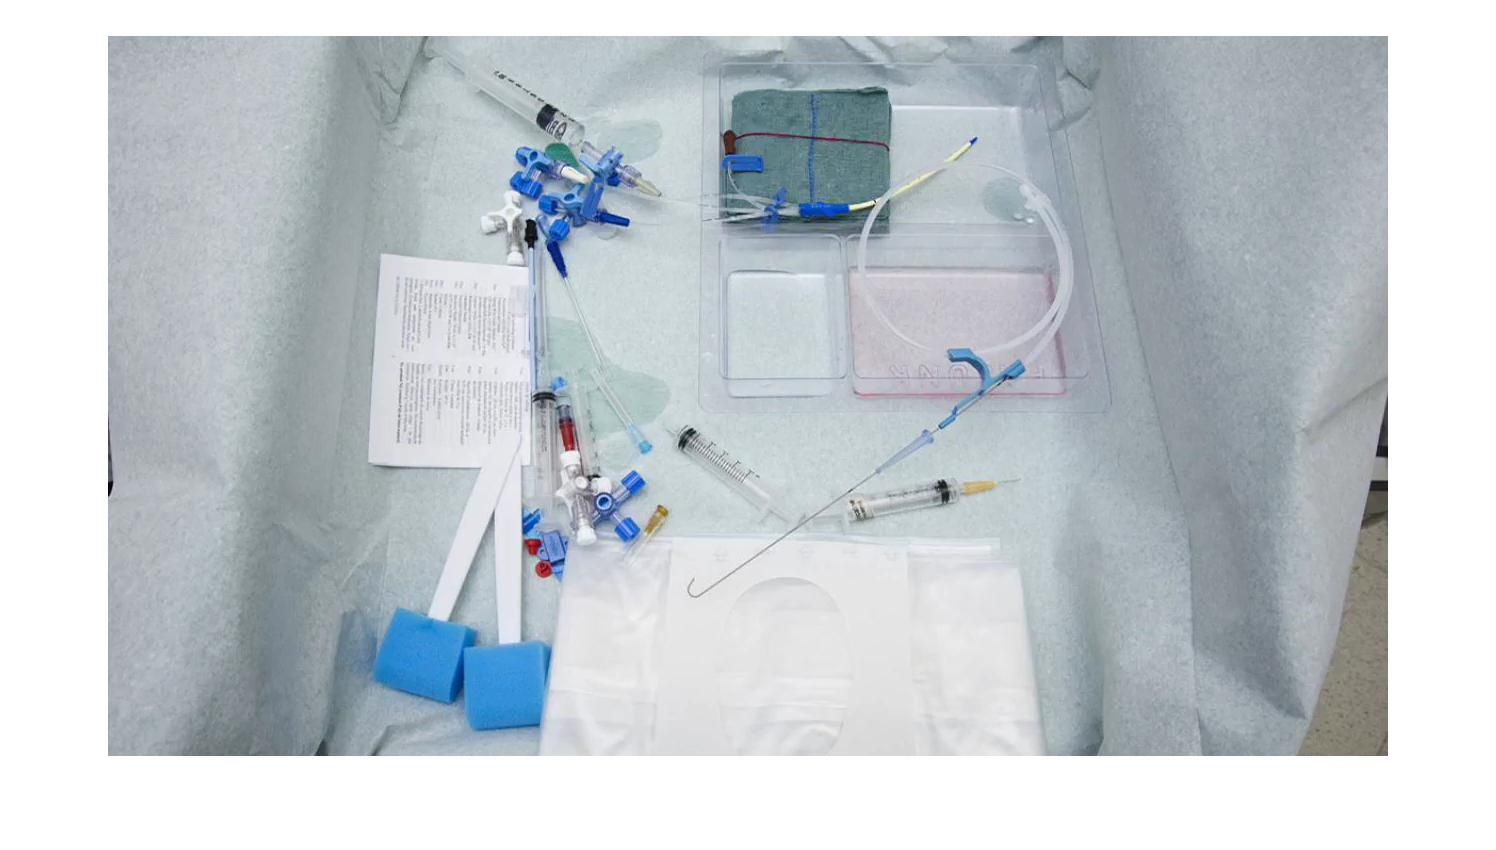
\includegraphics[width=10cm]{clip1.jpg}
				\centering
				\caption{A surgical equipment tray, with spillage under the needle}
			\end{figure}
			The data collection from the previous research project was based around a supervised eye tracking experiment in which a mixture of Expert and non-Expert Anaesthetists were asked to view a sequence of videos\cite{ameen}. These videos each depicted a scenario common to the practise, viewing an ECG screen, a surgical equipment tray etc., with a noticeable medical error in each. The subjects were prompted at the beginning of the exercise to look for these errors. These videos were compiled into a video exercise lasting approximately 5 minutes 30 seconds. The goal of the exercise was to elicit responses in experts and non-experts that differed from each other. The different responses would be represented in the subjects gaze data recorded by the Tobii eye tracking machine while the exercise is carried out.
			
			During the project previously carried out by the author, the gaze data was preprocessed, filtering out variables that did not seem relevant to this problem, these were measurements taken by the Tobii camera and didn't serve a purpose for observing the subjects gaze. The resolution of the gaze data was also scaled to fit the background image for visualisation.
			
	\chapter{Approach}\label{approach}
		The solution for this problem documented in this report focuses on feature extraction from the Tobii gaze data files. These features are then reduced in dimensionality into a linear combination that helped visualise any distinction between the two groups. The lower dimensional data is supplied to a SVM model that uses cross-validation to fit a margin of optimal separation to the feature-transformed data between experts and non-experts.
		\section{Quality of the data, and it's effect on results}\label{approach:dataquality}
			As stated above\ref{bg:previous} during the project in which the data was gathered, 15 subjects were recorded as they sat through the exercise. This is much smaller than generally accepted in machine learning, with the smallest number of samples expected to be in the 100s \cite{effectofdataset}. The lack of observed examples for either class might negatively effect the results of classification, as the outline of the space inhabited by either class in feature space will very likely not be defined well. This can be tackled by implementing oversampling, interpolating the data in order to get estimations of similar of observations at random\cite{oversampling}. 
			
			It must also be accounted for that the imagery used in the exercises may not be effective in eliciting different responses in experts and non-experts. In this case the features extracted and the classification model applied to the data will be unsuccessful for the most part no matter what method used, as the data itself has been recorded in a situation where the experts are not supposedly viewing the scene in a manner different to the non-experts.
			
		\section{Data Preprocessing}\label{approach:datapreproc}
			Gaze data files as recorded from the Tobii eye machine come in a particular format. The machine provides a large amount of information, most of which was not used in this project. The Tobii camera gives readings for the following:
			\begin{multicols}{2}\label{item:measures}
				\begin{itemize}
					\item{Timestamp}
					\item{Number}
					\item{GazepointX (L)}
					\item{GazepointY (L)}
					\item{CamX (L)}
					\item{CamY (L)}
					\item{Distance (L)}
					\item{Pupil (L)}
					\item{Validity (L)}
					\item{GazepointX (R)}
					\item{GazepointY (R)}
					\item{CamX (R)}
					\item{CamY (R)}
					\item{Distance (R)}
					\item{Pupil (R)}
					\item{Validity (R)}
				\end{itemize}
			\end{multicols}
			Of these, only Gazepoints L and R, Timestamp and Number were used for the purposes of this project. Timestamp and number act as indices for the gaze point, timestamp gives the time in milliseconds at which the frame recorded, and number is the number of the frame in the entire set collected for the exercise. Gazepoints L and R are both $x$ and $y$ coordinate pairs denoting the eye tracking cameras estimated position of the gaze on the screen. By taking the centre-point of both the $x$ and $y$ values, the subjects point of focus can be estimated for that frame. As a result the data was preprocessed, by filtering out these unnecessary measurements, before even clustering took place in order to make the information more readable for debugging. This results in a conversion from a table of 16 measurements to a set of $x$ and $y$ value pairs.
			
			The exercise originally contains all videos in sequence as one long video. By counting the frame index at which each clip starts within the video. These were then converted to the starting time in seconds. All timestamps are then collected into an array which is used to filter out the subset of coordinates that is relevant to the current clip. Finally, the resolution the data was recorded in by the Tobii camera is 1280x1024, whereas the first 6 clips showing images are 1280x720, and the last 8 showing videos of ECGs are 720x368. Therefore, before overlaying the gazepoints, in the tracking overlay or during clustering, the gaze data must be scaled down appropriately.
			
			Finally, the framerate of each video has been upsampled to fit the framerate of the Tobii machine, the gaze data is not affected therefore no information is lost. The only function of this is for data visualisation.
		\section{Exploratory Data Analysis}\label{approach:datavis}
			\subsection{Eye tracking overlay}\label{approach:datavis:overlay}
				\begin{figure}[h]\label{fig:eyeoverlay}
					\includegraphics[width=8cm]{eyeoverlay}
					\centering
					\caption{The first clip from the video, with the left (red), right (blue) and centre(black) gaze points of an expert}
				\end{figure}
				It seemed best to visualise the data first, in the hopes that a difference in the subjects' viewing habits would be made plain. By overlaying the gaze data per frame of the eye tracking file on the corresponding frame of the video \ref{approach:datavis:overlay}, it was possible to follow the subjects gaze and by comparing and contrasting subjects for different clips, any difference in viewing behaviour should become plain. 
				
				This view of the data was important as early on, it was intended for a Hidden Markov Model (HMM)\cite{hmm} to be fitted to each clip so that given a model for the clip it would be possible to separate any outliers, subjects who didn't behave as expected by the model, into a separate class from those who did. This did not prove viable as from the videos it was clear that while experts may spend the same time in certain areas of the screen, they did not visit each area in the same sequence, a characteristic necessary to HMMs.
			\subsection{Gaze Data Clustering}\label{approach:datavis:clustering}
				\begin{figure}[h]\label{fig:expertcluster}
					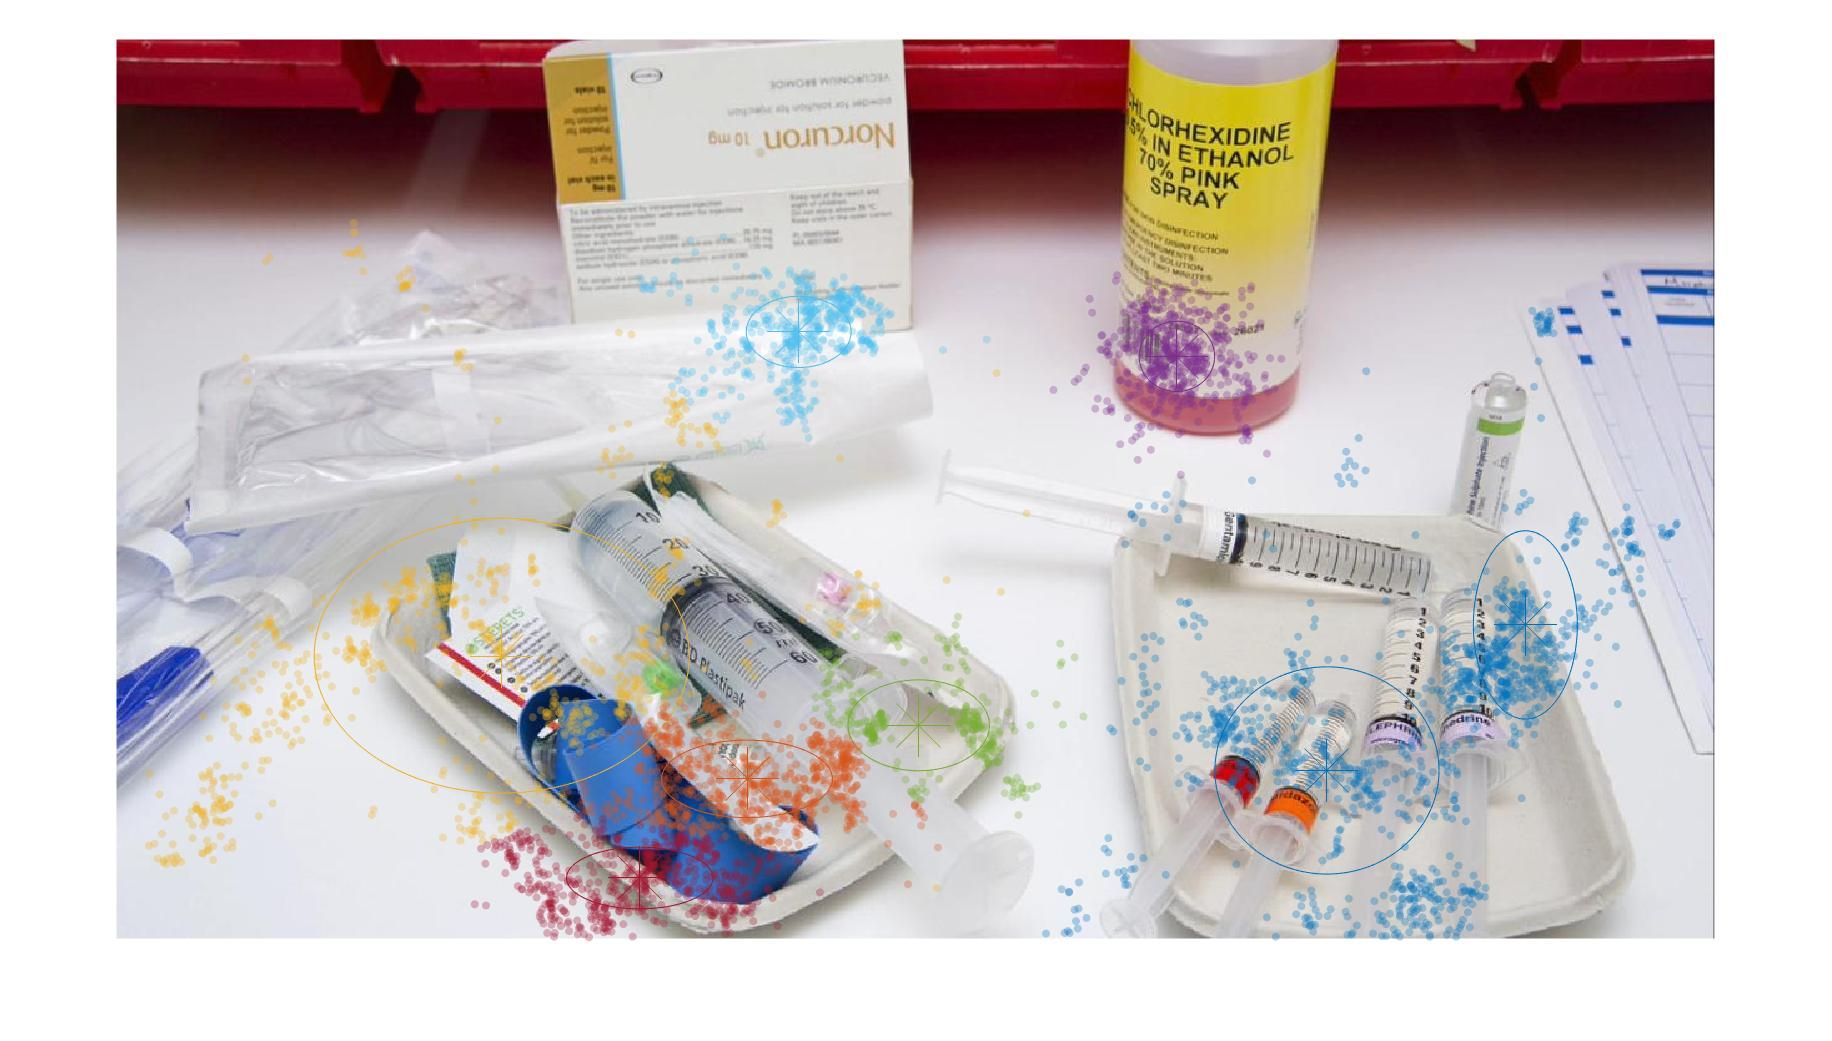
\includegraphics[width=10cm]{expertcluster}
					\centering
					\caption{Here the eye tracking data for all experts as they viewed the 3\textsuperscript{rd} clip is clustered using GMMs}
				\end{figure}
				A second approach was to cluster the gaze data of one group together over all the clip on to a freeze frame of the clip. Since the first 6 clips within the exercise video were scenes displayed in static images, the background was not temporally significant, and subjects from the same group could be compared together in order to create a heat map of sorts. For clustering, the k-means clustering algorithm was originally used. However, the clusters would often overlap or envelop smaller clusters entirely. k-Means clustering works by fitting the $n$ observations into $k$ sets \(S = \{S_{1},S_{2}, ..., S_{k}\}\), then minimising the variance per set\cite{kmeans}.
				
				The relatively poor clustering can be attributed to the k-means algorithm, due to its unsuitability for this data, as clusters in the gaze data are rarely circular. A different technique of clustering using a Gaussian Mixture model was much more suited as, rather than a hard border being fitted to each cluster, it instead fits a Gaussian blob\cite{gmms}. The implementation first fits cluster centres using the k-means algorithm, but then assigns data to Gaussians centred around these points. By measuring the posterior probability of a gaze point belonging to each of the Gaussians in the model, a membership to that Gaussian could be assigned to that point. This accounts for points that are on the margin of two clusters for example.
				
				A GMM was then fitted to a groups data for each clip, resulting in 28 models. One requirement of clustering is to provide the number of centres to be fitted to the data. This could quite easily make the difference between good and bad clustering as assigning an incorrect number of centres could lead to two clusters being misidentified as one, or one Gaussian enveloping all other data and containing any points too far from other centres to be considered as part of them, for example. However, rather than specify the number of centres based on how many clusters could be identified individually in each of 28 images, it was easier to implement a heuristic using the elbow method\cite{elbow} by incrementally increasing the number of centres, measuring the percentage of variance explained and defining a cut-off point where the gradient suddenly decreases (giving the appearance of an elbow in the graph. Percentage of variance explained is defined as the ratio of between-cluster variance to overall variance.
				
				One significant drawback with this approach to the data visualisation however, was that 7 of the 14 clips were video clips, featuring temporally dynamic stimuli, in the form of waveforms on an ECG. As the point of focus would likely move with the stimuli, removing the temporal aspect from the data would result in clusters that spanned the length of the waveform section on the screen, giving little insight into focus in a spatial respect around the crest of the wave.
				\begin{figure}[h]\label{fig:videocluster}
					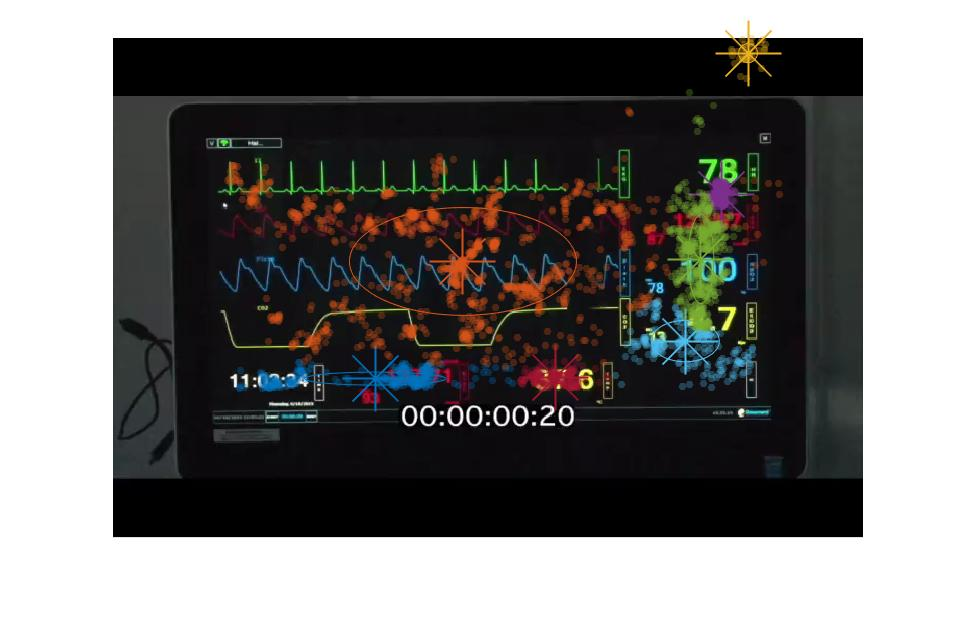
\includegraphics[width=10cm]{videocluster}
					\centering
					\caption{Poor clustering in the clip 7 due to objects moving along the screen}
				\end{figure}
		\newpage
		\section{Feature Extraction}\label{approach:ftextrac}
			Classification on the raw gaze data alone is implausible. This is because both groups would visit the same areas in the image, quite possibly at the same time, as all stimuli in the image do not require any expertise to notice. Rather, it is in understanding them the distinction between groups would lie. Practically this means on a two dimensional space (the eye tracking data) both groups would be indiscriminable, making the task of finding a hyperplane between them meaningless. However, so long as behaviour of subjects sharing a group is similar, and as a whole different from subjects in the other group, feature extraction should provide significantly separable groups of subjects, matching their class.
			
			Also while an experts activity over the whole clip might not be meaningful enough for classification, how their activity changes over the duration of the clip could prove significant. For instance, given an experts likely familiarity with the scenes displayed in the exercise, it is logical to assume that they are able to process the apparent information faster, and they might quickly scan the clip and then rest for the remainder of the clip. For this reason each feature was measured 15 times over each clip, once per second.
			\subsection{Definition of a fixation}\label{approach:ftextrac:fixationdef}
				Many of the features defined in this project are statistics concerning the subjects behaviour while fixating. The definition of a fixation used for this purpose follows an algorithm that filters out fixation points based on a set of criteria, if their velocity is lower than a cut-off velocity and if they are surrounded by other gaze points that pass the first condition as well. This algorithm is better defined in a paper on user attention\cite{overtva}:
				\begin{enumerate}\label{enum:fixationdef}
					\item{Calculate point-to-point velocity for each sample: }
					\item{Label each sample below 25$^{\circ}s^{-1}$ as belonging to a potential fixation period, otherwise as to a saccade period.}
					\item{Merge consecutive potential fixation period samples into a fixation group, removing saccade samples. The length of these groups, or in other words the fixation duration, must be higher than $$100ms$$. Under this threshold, the samples belonging to either a saccade or short fixation group, are discarded;}
					\item{Compute the spatial coordinates of each visual fixation (as the gravity centre of the coordinates of the samples in the considered group).}
				\end{enumerate}
				This algorithm was nicely translatable into the projects application, with a few approximations. Firstly, to measure $100ms$, it was necessary to calculate the framerate of the Tobii camera, and then the number of frames recorded by the camera in $100ms$. The framerate can be calculated using the total number of frames of eye tracking data \(N_{F}\) for one subjects exercise, divided by the time elapsed in seconds during the exercise, \(T\).
				\[\frac{N_{F}}{T} = \frac{16073}{320.362s} \approx 50s^{-1}\]
				At $50fps$, 5 frames will transpire in $100ms$. The algorithm was modified to include this, i.e. a group of potential fixations must last longer than 5 frames. 
				
				The second step was to calculate movements under 25$^{\circ}$/s. Using trigonometry to calculate the number of pixels per degree, made this a matter of conversion. The physical size of a pixel depends on what's known as the Dots per inch, or DPI of a screen. Monitors fall into categories for DPI, which are easily available online \footnote[1]{https://snapshop.cam/dpi/}. Estimating the size of the monitor used, and with knowledge that it was standard issue IT equipment for hospital staff, it seemed reasonable to settle on 72DPI, a figure confirmed by medical supervisor Dr. Lim. By making approximations of the distance the viewer sat from the screen, and assuming a sitting distance of $45cm$, or $17.71654in$ the distance travelled by the gaze in pixels as a result of turning the eye 25$^{\circ}$ is:
				\[d_{px} = \lvert{\frac{17.71654 tan(25)}{72}}\rvert \approx 170.32px\]
				Therefore, \(1^{\circ} = \frac{170.32}{25} \approx 7px\).
			
				For features that used the cluster of the gaze point, it was also necessary in the algorithm for a fixation to remain in the same cluster for it's duration.
				
			\subsection{Assigning clusters}\label{approach:ftextrac:choosingcluster}
				When assigning each data point to a cluster, the expert model was used for each clip. The expert clustered much more nicely, and better defined the objects in the scene. This also suited a larger decision made whilst designing the classifier \ref{approach:class}.
				\begin{figure}[h]\label{fig:clustercomparison}
					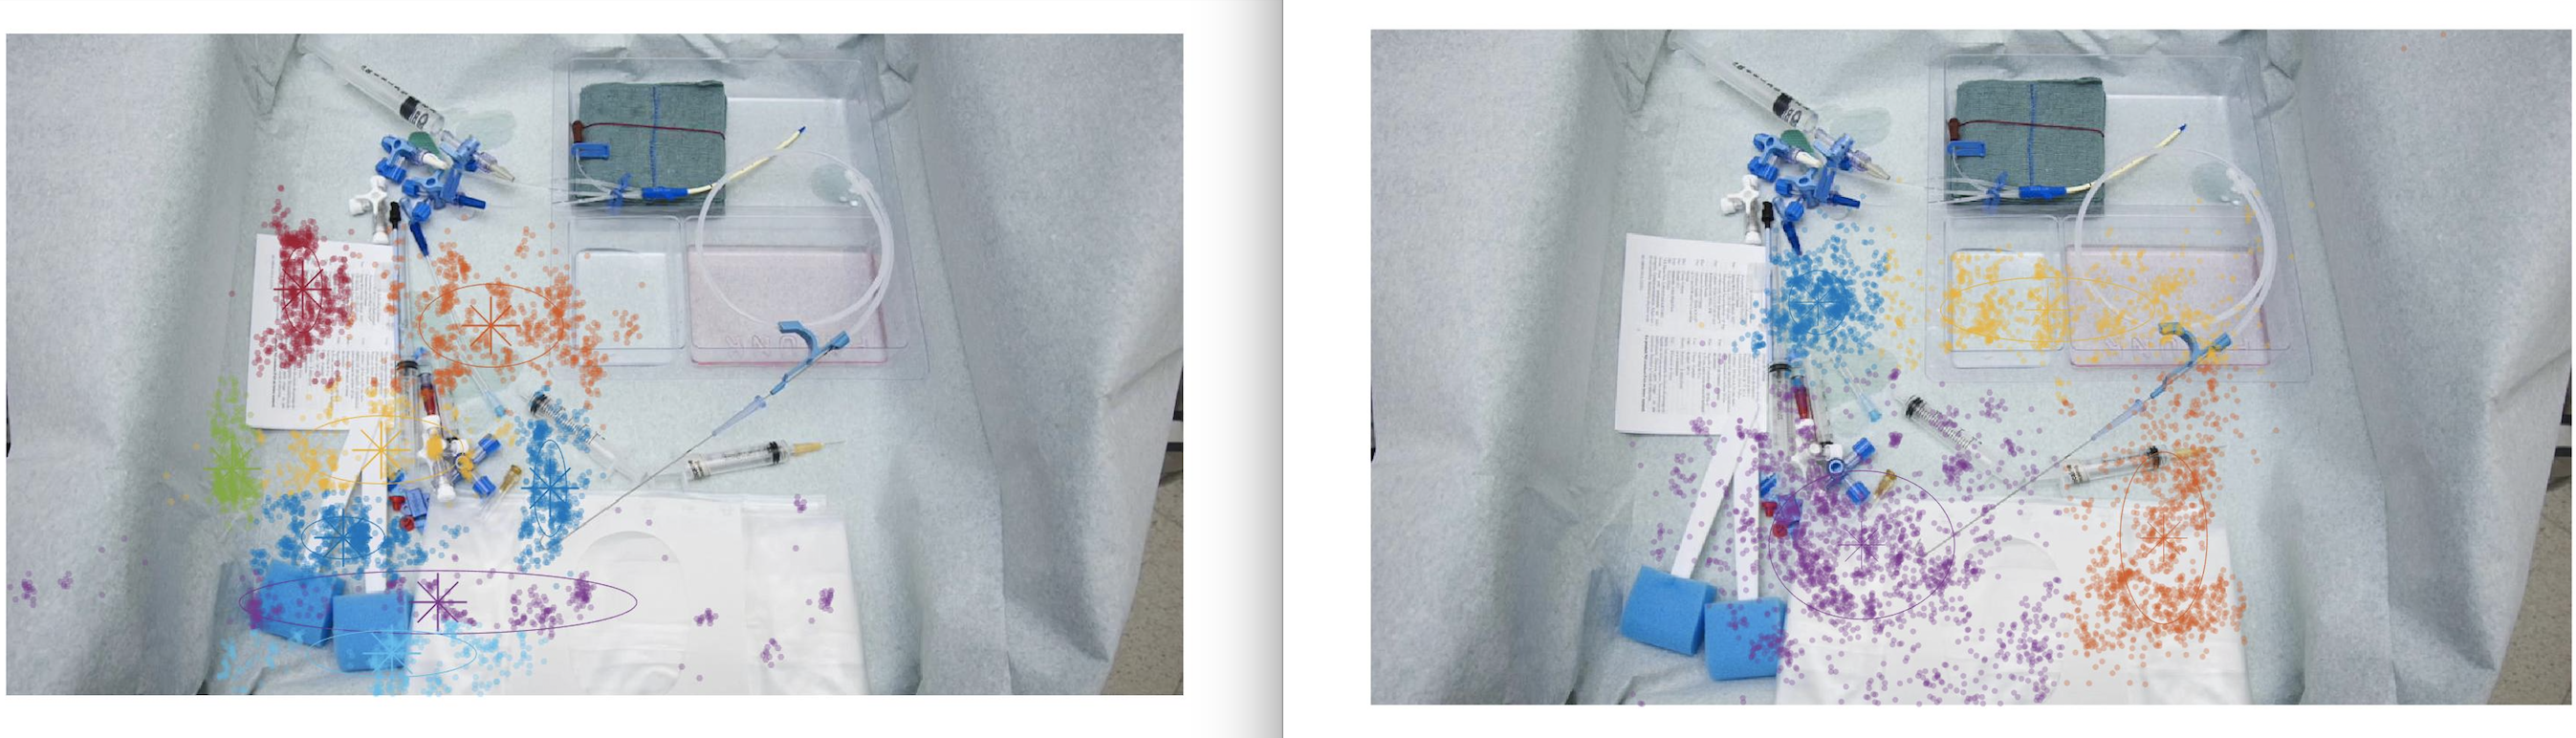
\includegraphics[width=12cm]{clustercomparison}
					\centering
					\caption{A side-by-side comparison of the clustering of expert (right) and lay (left) data shows that expert clusters span much more of the screen and demarcate well defined regions within the scene, whereas lays only cover one half of the screen}
				\end{figure}
				
			\subsection{Spatial features}\label{approach:ftextrac:spatialft}
				Spatial features are measures of how the subject moves around the screen, for example the distance travelled in the exercise by the gaze around the screen.
				
				Experts seemed to demonstrate a much more steadier focus while fixating as opposed to lays who exhibited more erratic movement. Therefore, the mean variance within a cluster for each second long section of the clip is used. This was measured along both $x$ and $y$ axes. 
				
				The frequency at which the experts would flick between different areas in the scene also appeared to be higher than that of the lays, who would meander through a path across the screen. Such behaviour would manifest itself as a huge difference in distance travelled, defining a second spatial feature.
				
				Another hypothesis that experts might accelerate more rapidly towards each cluster, as they recognised and honed in on the stimuli at the center of that cluster is also tested.
				
				As another feature, the total number of transitions made from one cluster to another is used, to which the observation of lays flicking between regions frequently lends confidence to.
				
				In summary, five spatial features were measured 15 times over a 15 second duration:
				\begin{itemize}\label{item:spatialft}
					\item{Average in-cluster variance in the $x$ direction.}
					\item{Average in-cluster variance in the $y$ direction.}
					\item{Total distance travelled by gaze.}
					\item{Average acceleration towards a cluster.}
					\item{Total transitions from one cluster to a different cluster.}
				\end{itemize}
			\subsection{Temporal Features}\label{approach:ftextrac:temporalft}
				Temporal features would describe how the subjects spend their time during the exercise, i.e. how long they focus on any particular thing, or how often they focus.
				\subsubsection{Cluster Features}\label{approach:ftextrac:temporalft:temporalcluster}
					Following the same logic used for Spatial features, it would stand that Experts would spend less time focusing on any area as they should recognise errors quickly from experience and training. This was translated to average duration spent in one cluster. However, as some of the clusters are quite large, with some covering around 30-40\% of the screen, it is possible that the gaze could remain in one cluster for an extended period of time without fixating for the most of that time. So the total number of fixations in a cluster was taken as an additional measure.
				\subsubsection{Non-Cluster Features}\label{approach:ftextrac:temporalft:temporalnoncluster}
					In order to account for unsuccessful clustering, as in the ECG clips, and behaviour that might not remain within a cluster, or where the cluster is not significant, it was also important to take a selection of temporal features that do not consider the cluster data, rather just measuring features from the raw gaze data.
					
					Time taken before the subject fixates at the very beginning of the clip was used to measure how quickly experts find and focuses on an object in the scene.
					
					The total number of fixations and the average duration of a fixation per section also seemed promising, based on the observation that Experts seem to hone in on objects and remain for longer, i.e. fixating less frequently and for longer. Similar to these features, is the time spent not fixating, with the hypothesis that Lays would spend more time scanning rapidly across the scene.
				\\
				\\
				In summary five suitable temporal features were found, again measured 15 times during the clip, excluding time to initial fixation, which was measured only once:
				\begin{itemize}\label{item:temporalft}
					\item{Cluster features}
					\begin{itemize}
						\item{Total number of in-cluster fixations.}
					\end{itemize}
					\item{Non-cluster features}
					\begin{itemize}
						\item{Time until initial fixation.}
						\item{Total number of fixations.}
						\item{Average duration of a fixation.}
						\item{Time spent not fixating.}
					\end{itemize}
				\end{itemize}
		\newpage
		\section{Dimensionality Reduction}\label{approach:dr}
			With 10 total potential features, with each feature measured and recorded 15 times per clip, classification would be in 150$^{th}$-dimensional space. This would then be increased by the SVM as the purpose of the kernel trick is to increase dimensionality of the data to find hidden separation (explained in \ref{bg:analysis:svms}).
			
			Therefore, although compiling a large number of features would increase the likelihood of finding a distinguishing relationship between the groups, it also increases the complexity of training and testing the resulting classification model. When implementing dimensionality reduction, using the correct method should reduce the complexity of the data with minimal loss of information. Two popular methods, t-SNE and PCA, have been chosen for data visualisation and analysis, and classification respectively.
			\subsection{t-SNE}\label{approach:dr:tsne}
				t-distributed Stochastic neighbour embedding is a non-linear dimensionality reduction method\cite{tsne}. In two stages, it fits a probability distribution to pairs of points in the high dimensional data such that similar points have a high probability, and that conversely dissimilar points have very low probability. A p.d. is then defined with lower (2\textsuperscript{nd} or 3\textsuperscript{rd}) dimensionality. The divergence of these p.d.s is then reduced such that similar points in the high dimensional data have mappings with similar probability in the lower dimensional representation. This method is particularly useful for data visualisation, as relationships between data are preserved in a visualisable dimension. However information isn't technically retained, as the probability distribution of similarity between points does not account for magnitude for instance. t-SNE can be performed using a variety of distance metrics, of which Cosine, Euclidean and Chebychev distance were used, for comparison. A fourth measure, Mahalanobis distance was not possible with this data as it requires that the covariance of the data be symmetric.
				
				The Cosine distance is defined as \(1 - cos(\theta)\) where \(cos(\theta)\)\ is the cosine of the included angle between observations (treated as vectors).
				
				Chebychev or chessboard distance is the maximum coordinate difference between points.
				
				Euclidean distance is described below.
				
				\begin{figure}[h]\label{fig:tsnedistance}
					Cosine Distance: \[ d_c (a,b) = 1 - cos(\theta) = 1 - \frac{\mathbf{A} \cdot \mathbf{B}}{\|\mathbf{A}\| \|\mathbf{B}\|} = 1 - \frac{\sum\limits_{i=1}^n A_i B_i}{\sqrt{\sum\limits_{i=1}^n A_i^2} \sqrt{\sum\limits_{i=1}^n B_i^2}}\]
					Euclidean Distance: \[ d_e(a,b) = d_e(b,a) = \sqrt{\sum\limits_{i=1}^n(b_i - a_i)^2}\]
					Chebychev Distance: \[d_{ch}(a,b) = \lim_{k\to\infty} \Big(\sum\limits_{i=1}^n\lvert p_i - q_i |^k\Big)^\frac{1}{k}\]
					\centering
					\caption{The mathematical formulas associated with the 3 distance measures used by t-SNE in this project}
				\end{figure}
			\subsection{PCA}\label{approach:dr:pca}
				Principal Component Analysis is a linear dimensionality reduction method, for data with multiple correlating dependent variables. In short, PCA transforms the data onto a new coordinate system that emphasises patterns and variance in the data\cite{pca}. It does this by projecting the data onto the new coordinate system such that the most variance in the data is on the first axis, the next most on the second and so on. 
				
				Intuitively, in a coordinate system where variance in the data is at it's greatest, finding separation between subsets of the data will be at it's easiest. It is for this reason that PCA lends very strongly to classification methods that separate the data, notably SVMs. As each of the new coordinates, or principal components, is a linear combination of the original axes, the dimensionality of the data is also reduced. 
				
				As the principal components are sorted in order of decreasing variance, by definition, selecting the first n principal components such that these account for more than say 90\% variance, means that any additional principal components can be discarded with only 10\% variance lost. This cut-off can be tweaked as appropriate, or can suit the number of desired dimensions. 
				
				However, data that is evenly spread, for instance circular, will result in relatively even distribution of variance between principal components resulting. In this scenario the resulting loss in variance would be significant enough for dimensionality reduction to be much less feasible. One other possible reason for evenly distributed variance is the clustering of the data into two or more sub groups, each with variance in different dimensions. By splitting the data using a GMM and measuring the explained variability of each PC in each Gaussian it can be determined if this is the case. If the variability in both Gaussians is heavily biased to the first PC then this possibility is likely true.
				
				Two matrices are conventionally outputted as a result of the PCA algorithm, the first, a set of coefficients or loadings, containing rows of coefficients for each column relating to a principal component. The loadings allow by matrix multiplication the conversion of data from the original feature space into principal component space. The second matrix is the converted data used to find the components. 
				
				In this project, PCA proved very effective not only for visualising relationships between data in a lower dimensionality, but also effectively providing a linear combination of the most distinguishing variables of data, along with a relatively simple means of converting any new data into this format.
				
				For classification, the process is similar, with each principal component taking the place of a variable. In the event that the principal components are split into two Gaussians, then a model is built for both subsets of the data, and the result is taken to be the average loss over both models.
		\section{Classification}\label{approach:class}
			Classification is the main objective of this project. There are various approaches that can be taken to classification in order to fully assess the plausibility of classifying expert and non-expert. Given 150 variables, it is simple to implement single variable classification as well as evaluate pairs of variables for classification. If the lack of observations, i.e. subjects, appears to affect the results too negatively, an oversampling approach can be applied to the data such that each observation is surrounded in feature space by a number of similar pseudo-random observations, interpolating the data but maintaining most information, as the points that are generated will be close to the originally measured points. Doing so will better define the space inhabited by both groups, in the hope that the model is misclassifying by a very small margin, in which case it will then misclassify half of the observations in that cluster rather than 100\%.
			\subsection{Single-variable and pairwise classification}\label{approach:class:singleandpair}
				Classifying using a single variable is a simple method for assessing that variables usefulness in the model. Since the dimensionality is as low as it can be and no preprocessing need occur before classification, it is prudent to test each variable. Secondly, by creating a heat-map of variables classified in pairs, weak and strong areas in classification could be visualised.
			\subsection{Sequential Forward Selection}\label{approach:class:sfs}
				A popular search method in feature space known as sequential forward selection is a useful heuristic for building an effective classification model. Sequential forward selection adds features from the feature space sequentially until the loss, which can be user defined, increases. The main drawback of this technique is that if poor features are ordered first, these will be added, increasing the loss, and therefore ending the process before better features can be added\cite{sfs}. Sequential forward selection becomes considerably more practical a method once the variables are sorted in order of descending accuracy, effectively allowing SFS to create a partition of useful and non-useful variables, where usefulness is determined by contribution to the classification models accuracy. A counterpart of SFS is sequential backward selection, which begins with a model including all variables, and incrementally removes them until the accuracy decreases.
			\subsection{Classification in Principal Component space}\label{approach:class:pca}
				As previously explained PCA is very useful for maximising the variance in the data. It is as a result of PCA that the potential separation between experts and non-experts in feature space is most defined, this should make the SVMs job considerably easier if in the original feature space separation is very slight.
			\subsection{Configuring hyperparameters}\label{approach:class:param}
				There are many hyperparameters in a SVM model that can be tweaked to better fit the scenario. The strongest and most apparent example being the kernel function used to transform the data into a higher dimensional space. There are three built-in functions available, namely linear, Gaussian or radial basis function and polynomial kernels. Each function is suited to a different application. For instance, the Gaussian kernel is default for one-class learning \cite{oneclasswGaussian}. The polynomial kernel is used in cases where data is not linearly separable in feature space but requires the order of polynomial used to be provided.
				
				The box constraint for the model also requires tuning. The box constraint is a measure of penalty on the model that encourages more separation by increasing the cost of misclassified observations in the training data. By increasing this value the model will be trained with stricter separation.
				
	\chapter{Implementation}\label{impl}
		This chapter documents the resources, libraries and implementation used to achieve the methods listed in approach.
		\section{Environment}\label{impl:devenv}
			This project's scope is with analysing and classifying previously collected data, and as such, no further data collection was required. The data that has been used has already been cleared for ethical approval, and therefore this is not a concern for this project. 
	The Software Implementation was developed and tested on a 2016 MacBook Pro with a 2.3 Ghz Intel i5 Core and 8 GB of memory, running MATLAB 2016b.
			\subsection{MATLAB}\label{impl:devenv:matlab}
				Matlab is a programming language tuned towards mathematical and scientific programs developed by Mathworks. With heavy focus on mathematical formula and data visualisation it is a very popular tool for data scientists and analysts\cite{matlab}. The development environment provides an intuitive means of debugging code. Matlab provides a variety of licensed toolboxes for additional functionality such as Machine Learning and Image Processing. As a result, the Matlab community has a heavy focus on scientists and academics, providing a lot of support in the scope that this project falls in. This all makes Matlab an excellent choice for this project as with the aforementioned Machine Learning Toolbox, along with various other external toolboxes and libraries provided by the community, the main goal of the project could be focused on with very little distraction in terms of ancillary functionality that would otherwise reduce the time available to carry out the necessary experiments documented in \ref{approach}.
		\section{Toolboxes and Libraries}\label{impl:toolbox}
			Many algorithms and methods necessary to the project approach have already been implemented, either officially by Mathworks or by the Matlab community. Implementations of clustering methods and dimensionality reduction for instance are outsourced in this project to available toolboxes.
			\subsection{Statistics and Machine Learning Toolbox}\label{impl:toolbox:statsandml}
				This official Matlab toolbox was essential for this projects success. Providing not only highly customisable methods for classification, but also clustering, data partitioning and dimensionality reduction.
				\subsubsection{Clustering}\label{impl:toolbox:statsandml:clustering}
					The function used for \texttt{kmeans} clustering can be found in this toolbox. The \texttt{kmeans} function takes as it's mandatory arguments the data in a matrix $x$ of n observations of p variables, and k, the number of partitions into which $x$ is split by the algorithm. As the clustering method was later changed to GMMs \ref{approach:datavis:clustering} the k-means method is not used in the final implementation of the solution.
				\subsubsection{Dimensionality Reduction}\label{impl:toolbox:statsandml:dr}
					Implementations of both t-SNE and PCA are both available through the Stats and ML toolbox. The \texttt{pca} function takes a matrix $x$ of n observations of p variables, and outputs 3 notable values. The loadings matrix \texttt{coeff}, the principal component scores in \texttt{score}, and \texttt{latent}, a vector of the explained variability of each principal component. 
					
					As mentioned before in \ref{approach:dr:tsne}, t-SNE can be used for data visualisation. The function \texttt{tsne} takes as its arguments, the matrix X, in the same format as \texttt{pca} and \texttt{kmeans}. It can also take Name-Value pairs, including 'Distance' followed by 'mahalanobis', 'cosine', 'chebychev' or 'euclidean'. Another notable optional parameter is 'NumDimensions' which is by default 2, but can also be 3 for 3 dimensional data representation.
				\subsubsection{Classification}\label{impl:toolbox:statsandml:class}
					The main and final goal of this project is successful classification of experts and non-experts. The Stats and ML toolbox provides a ClassificationSVM class, with methods for fitting, \texttt{fitcsvm}, and predicting, \texttt{predict}, a SVM model. There are also methods for cross evaluation, \texttt{crossval}, and finding the estimated loss of the model, \texttt{kfoldLoss}. Additionally, this toolbox provides the implementation of SFS used in this solution.
			\subsection{NETLAB}\label{impl:toolbox:netlab}
				The NETLAB toolbox provides various functionality for pattern recognition. It was suggested for the project as a solution to the poor clustering provided by the k-means algorithm as it contains an implementation of Gaussian Mixture models for clustering data. The GMM code consists of several functions (gmminit, gmmpost etc.) that allow the creation, initialisation, fitting and EM training of a GMM. These were possibly the most used out of all methods used for data preprocessing and analysis, being at least on par with the SVM methods for use. In the NETLAB implementation, a GMM is created with the function gmm, taking parameters for number of dimensions, number of centres and type of covariance matrix. The model can then be initialised on a data set using gmminit before finally being run through the Expectation Maximisation, or EM algorithm to fit the model to the data.
			\newpage
			\section{Algorithms}\label{impl:algorithm}
				This section documents the implementation in Matlab of some of the algorithms listed in \ref{approach}.
				\subsection{Data Preprocessing}\label{impl:algorithm:datapreproc}
					While this code was developed as part of the previous project in preprocessing the gaze data, it is noteworthy as it scales and filters the gaze data from its raw format.
					\lstinputlisting[caption = {This code filters out data for the specific clip, using an array of timestamps, and the clip no. taken as an argument. It then scales the resolution down depending on the clip.}]{scaledata.m}
				\newpage
				\subsection{Data Analysis}\label{impl:algorithm:analysis}
					\subsubsection{Overlay}\label{impl:algorithm:analysis:overlay}
						In order to visualise the tracking data overlaid on the background clip, an algorithm that would plot the data as points, on the same figure as the image, for each frame was necessary. In order to better visualise the movement, a line between the previous and current gaze points is plotted, giving the appearance of gazepoints leaving a short trail as they move. 
						\lstinputlisting[caption = {This code provided the initial data visualisation necessary to disproving the feasibility of using HMMs \ref{approach:datavis}}]{overlay.m}
					\newpage
					\subsubsection{Clustering}\label{impl:algorithm:analysis:clustering}
						The final incarnation of the clustering algorithm used in this solution is a combination of clustering using GMMs repeatedly, incrementing the number of centres, until the rate of change of explained variance per cluster decreases past a cut-off point, in what's known as the elbow method. The implementation of which is featured below.
						\lstinputlisting[caption = {Here, the number of Gaussians is increased every iteration until the error of the GM model increases by at least 1}]{elbowmethod.m}
				\newpage
				\subsection{Dimensionality Reduction}\label{impl:algorithm:dr}
						While t-SNE simply required plugging in via \texttt{tsne}, PCA although similar, requires mention as in the case of the data clustering, an algorithm to split the data into two Gaussians has been implemented.
						\lstinputlisting[caption = {The code repeatedly generates a Gaussian Mixture Model to fit the data until one is successful, then the observations are allocated to one of two centres based on posterior probability}]{splitpca.m}
				\subsection{Classification}\label{impl:algorithm:class}
					\subsubsection{Classification on a single variable}\label{impl:algorithm:class:single}
						By evaluating each variables independent performance, not only is that variables usefulness in the end model assessed, but this also aided the sequential forward selection approach as variables could be sorted in descending order of accuracy.
						\lstinputlisting[caption = {Each variable, represented by a column of the data, is used to fit a 1 dimensional SVM, which is then cross validated, and the loss for that model estimated}]{singleft.m}
	classification on features as a whole
					\subsubsection{Variable pair classification}\label{impl:algorithm:class:pair}
						Evaluating variables in pairs produces a heat map of classification that is very useful for visualisation of the feature space for a clip. While computationally intensive to fit and cross validate a model for each possible pair of variables, the benefit the visualisation gives for evaluating a clip makes it a worthwhile endeavour.
						\lstinputlisting[caption = {An n-by-n matrix is generated for n features. The use of nested loops increases the complexity notably.}]{pairwise.m}
					\subsubsection{Sequential Forwards Selection}\label{impl:algorithm:class:sfs}
						The SFS algorithm required the creation of a cross validation object and a custom function that calculates a criterion value to be minimised.
						\lstinputlisting[caption = {The criterion function is passed to \texttt{sequentialfs} which generates multiple XT, Xt, yT and yt from the crossvalidation object c}]{sfs.m}
					\subsubsection{Classification in PC space}\label{impl:algorithm:class:pca}
						The final method of classification is in PCA space. The implementation shown also displays the method of oversampling data in the case that classification is poor. This precaution ensures that the space defined by experts and non-experts, if distinct, is as well outlined as possible. This means that if the hyperplane falls very slightly under one actual observation, the model loses say 59\% of the points in that cluster, rather than 100\%. 
						\lstinputlisting[caption = {Oversampling is achieved by randomly assigning a close by point to one of the actual observations, 100 times over for both experts and non-experts. This converts individual points into large clusters that should hopefully merge together}]{pcaclassification.m}
						
	\chapter{Results}\label{results}
		Both the distinct behaviour of experts and non-experts observed in the overlaid videos, and the clear difference between experts and non-experts in some features extracted \ref{approach:ftextrac} promised good classification. While this was not true in the original feature space, with some extra processing steps, using PCA data, very high accuracy was obtained on average for all clips.
		\newpage
		\section{Clustering}\label{results:clustering}
			\begin{figure}[h]\label{fig:goodcluster}
				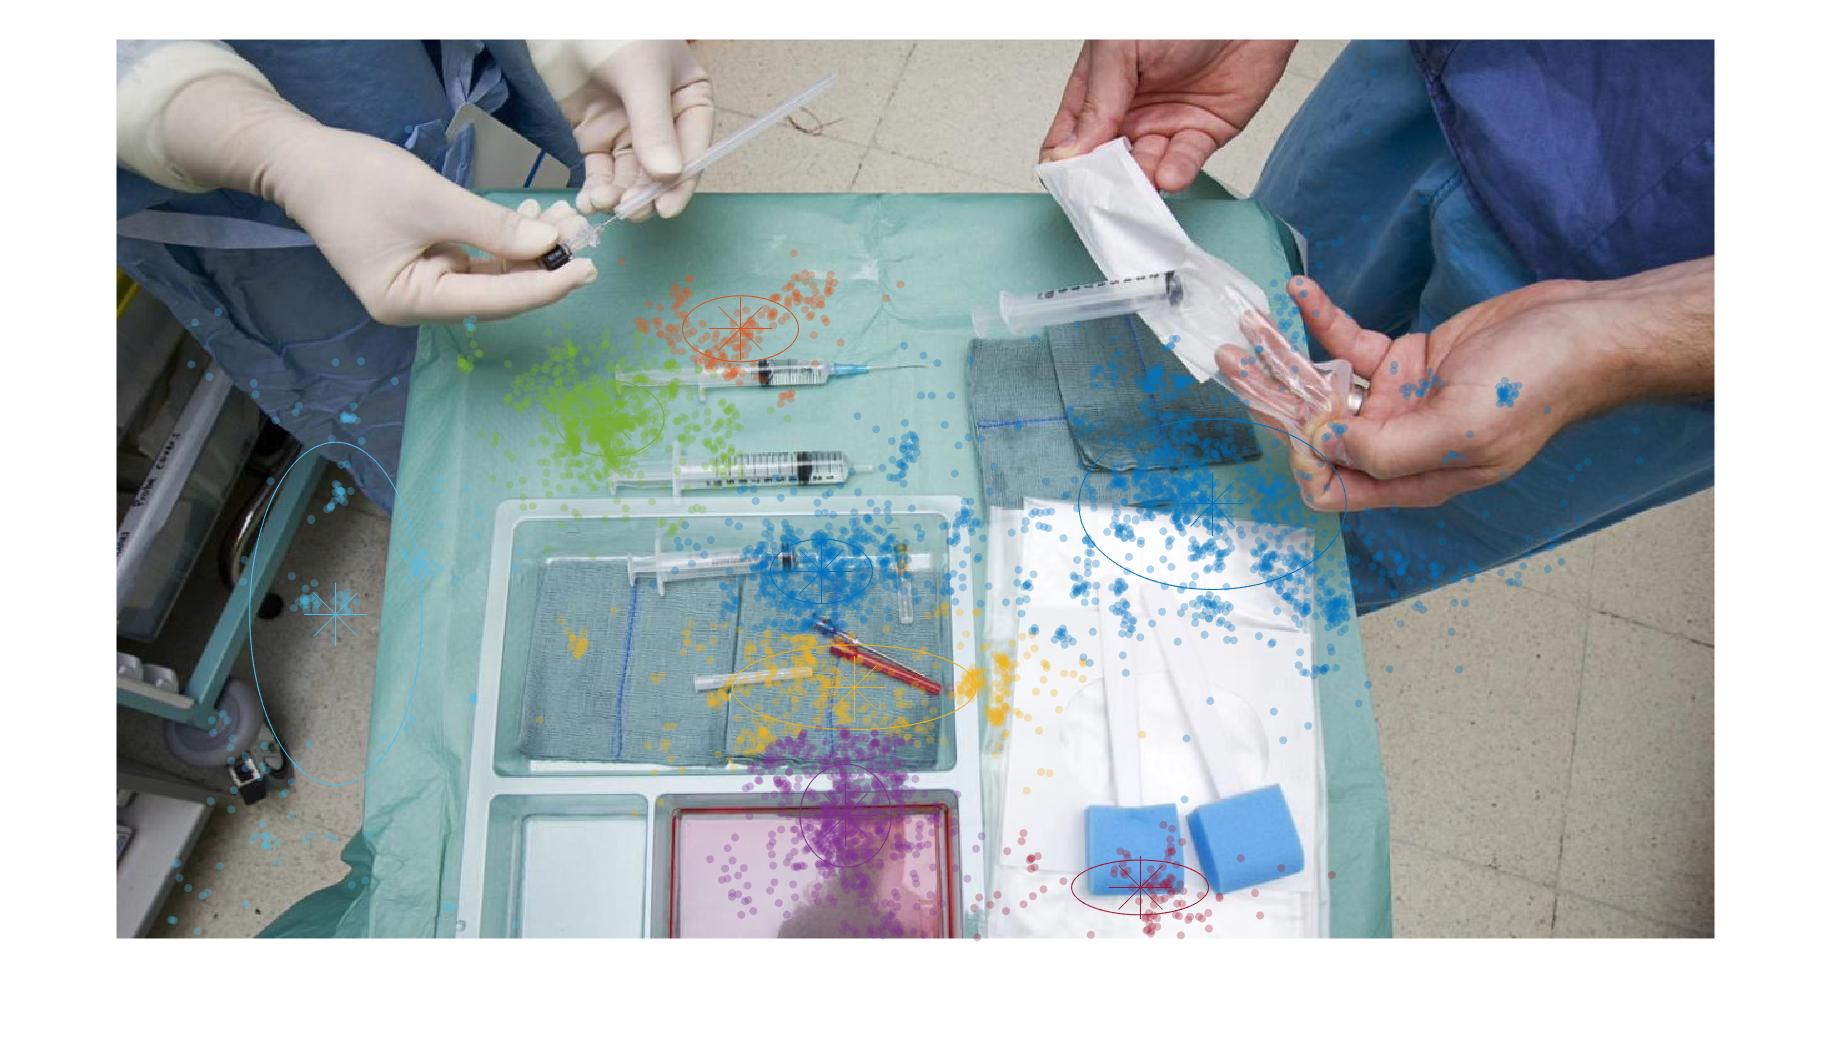
\includegraphics[width=8cm]{goodcluster}
				\centering
				\caption{The clustering here is for Experts whilst viewing the 2\textsuperscript{nd} clip. The gaze data defines isolated areas in the image well.\label{fig:gdcluster}}
			\end{figure}
			Generally the data clustered well. Applying the GMM approach to the gaze data resulted in an effective heat map for each clip based on an expert's gaze. Clusters overlapped very rarely and each cluster could consistently be definitively assigned to a group of objects. The significance of the clustering was less in the ECG clips, but altogether this provides a useful insight into the popular areas in the scenes.
			\newpage
		\section{Feature Extraction}\label{results:ftextrac}
			All features were used in the resulting model excluding Acceleration to cluster. This feature varied so distinctly between subjects in the same group that it was excluded in the final model \ref{fig:acc}.
			\begin{figure}[h]\label{fig:acc}
				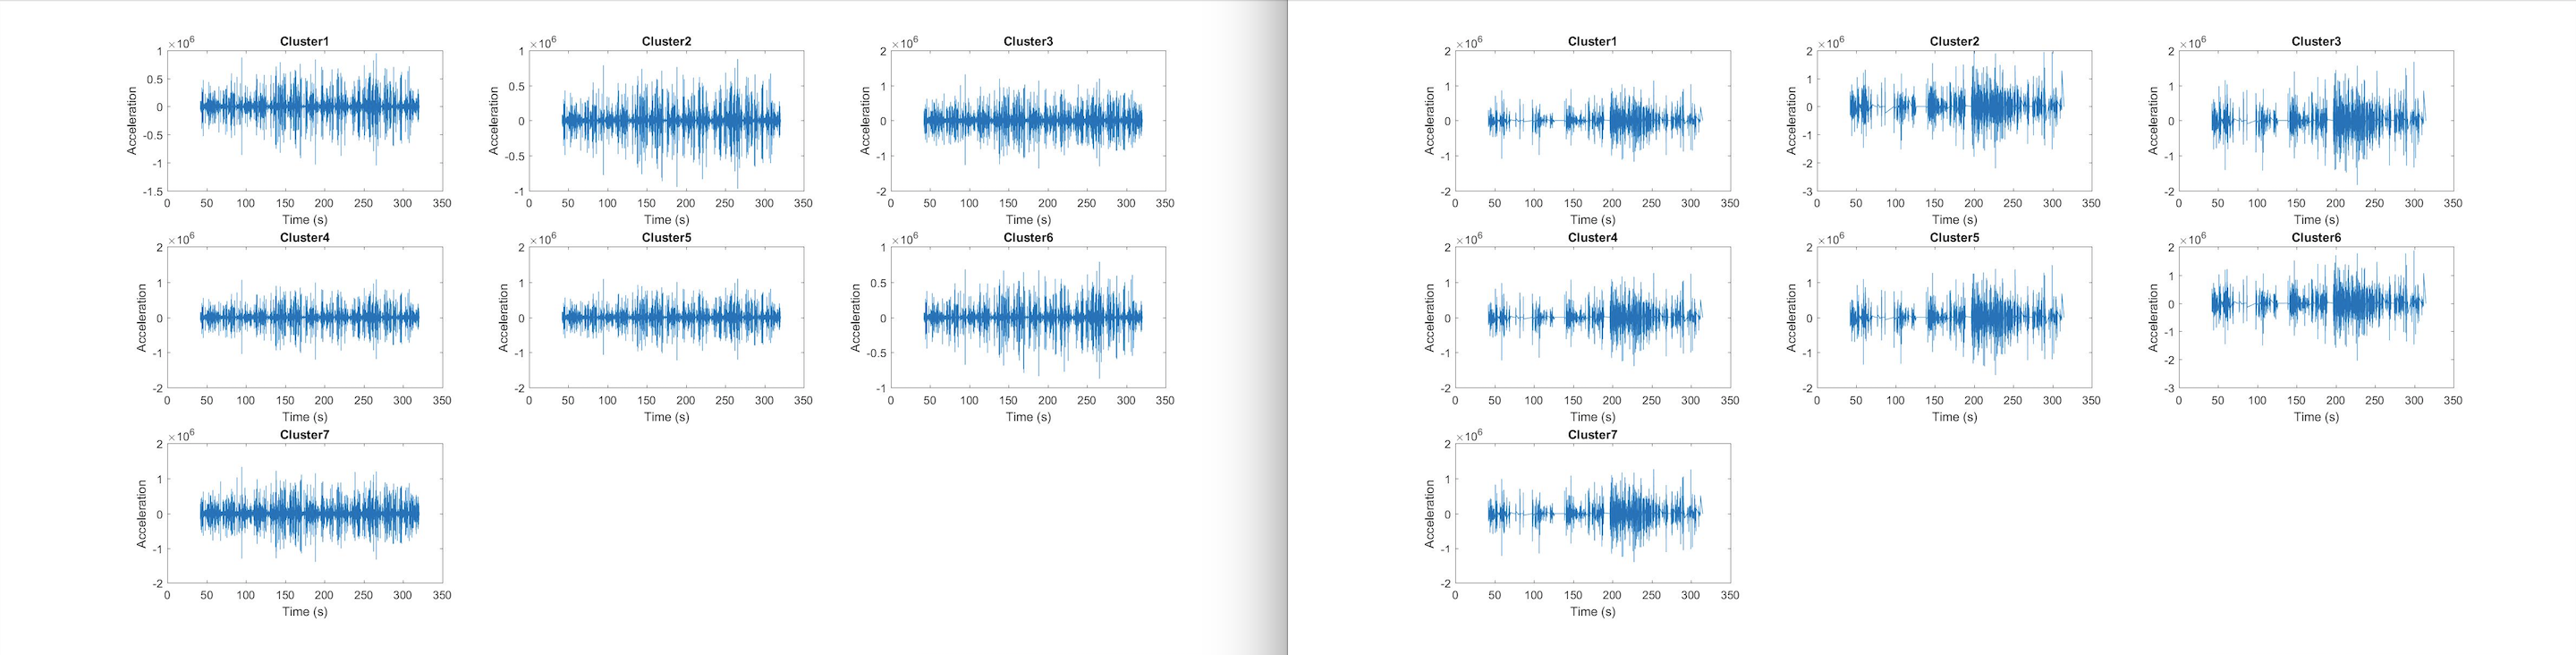
\includegraphics[width=15cm]{acceleration}
				\centering
				\caption{A side-by-side comparison of two experts accelerations to clusters demonstrates that the feature does not distinguish subjects as expert or non-expert}
			\end{figure}
			All other features seemed to demonstrate a pattern in subjects from different groups and were included in the classification analysis \ref{fig:distanceplot}. This leaves 121 features for classification in the final models for clips 1-6 \(((8\times15)+1)\), and 61 features for clips 7-14 \(((4\times15)-1)\).
			\begin{figure}[h]\label{fig:distanceplot}
				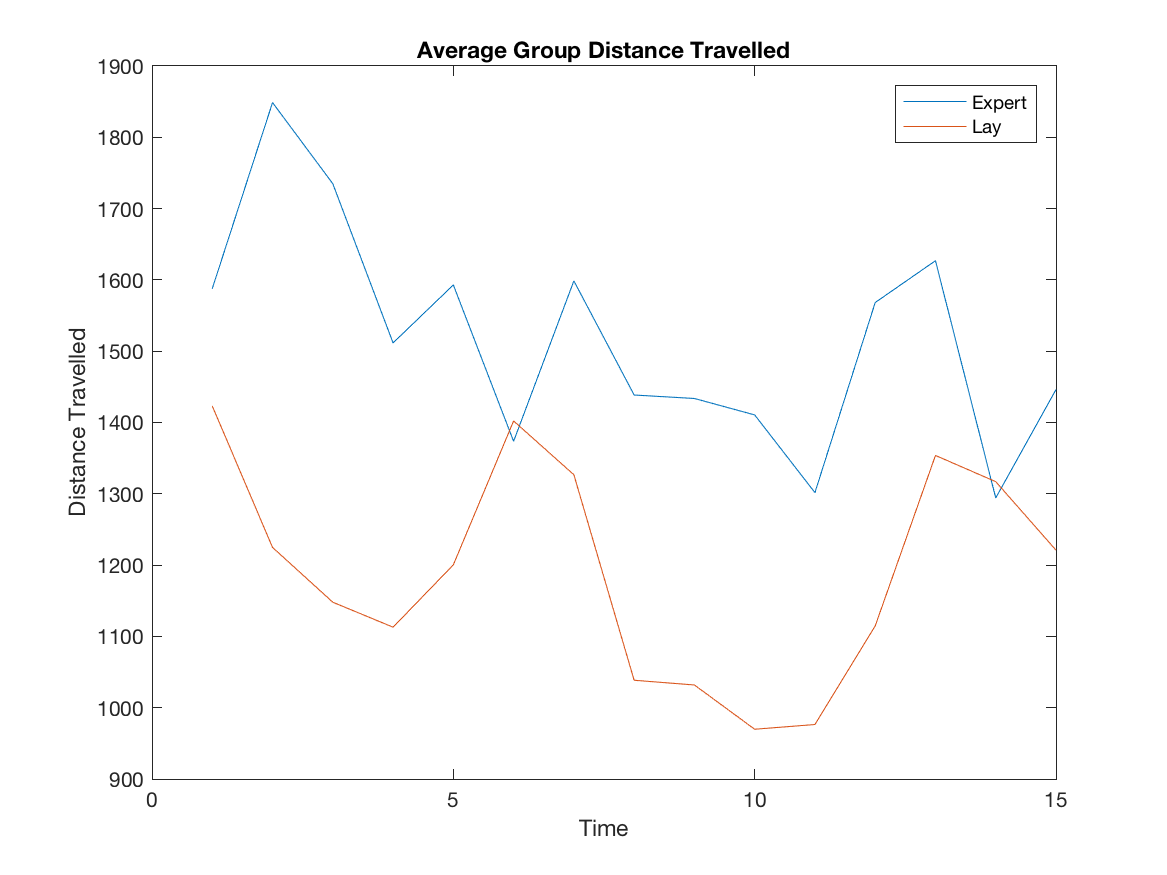
\includegraphics[width=8cm]{distanceplot}
				\centering
				\caption{Total distance travelled for an average expert vs non-expert shows that an experts gaze on average travels further than that of a non-expert}
			\end{figure}
		\section{Dimensionality Reduction}\label{results:dr}
			\begin{figure}[h]\label{fig:tsne}
				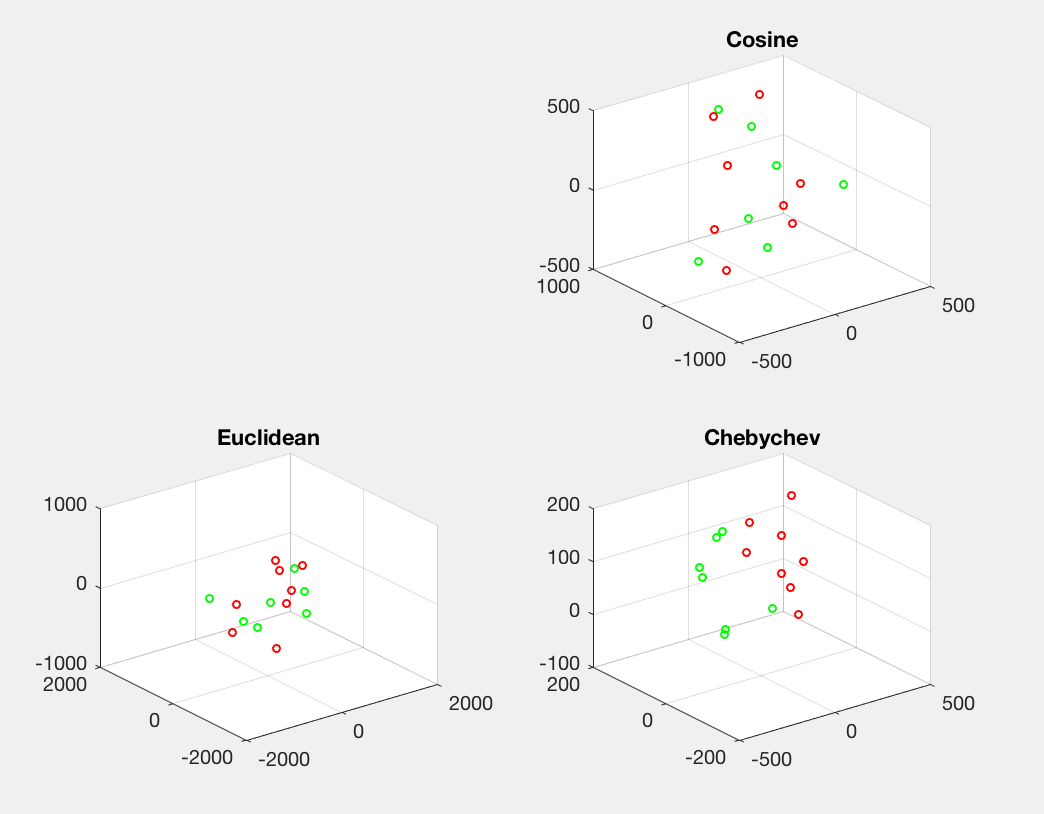
\includegraphics[width=8cm]{tsne}
				\centering
				\caption{The only representation in which the groups are clearly separated for clip 1 in 3 dimensions is Chebychev distance}
			\end{figure}
			The results of t-SNE were not very promising. Using all 3 possible distance measures separation did not appear to be a trait of this dataset. This does not mean the data is inseparable, however the only distance measure to translate the data into a lower dimensionality and retain a distinct border between the two groups was Chebychev distance \ref{fig:tsne}, although this was not the case for all clips.
			
			As stated in \ref{approach:dr:pca}, when PCA results in particularly evenly distributed variance between principal components, it is necessary to evaluate the explained variance of components split into a cluster. This proved true for all clips. It has become apparent variables commonly divided the data into two groups, such that both groups displayed variance in a different set of variables.
			\begin{figure}[h]\label{fig:splitpca}
				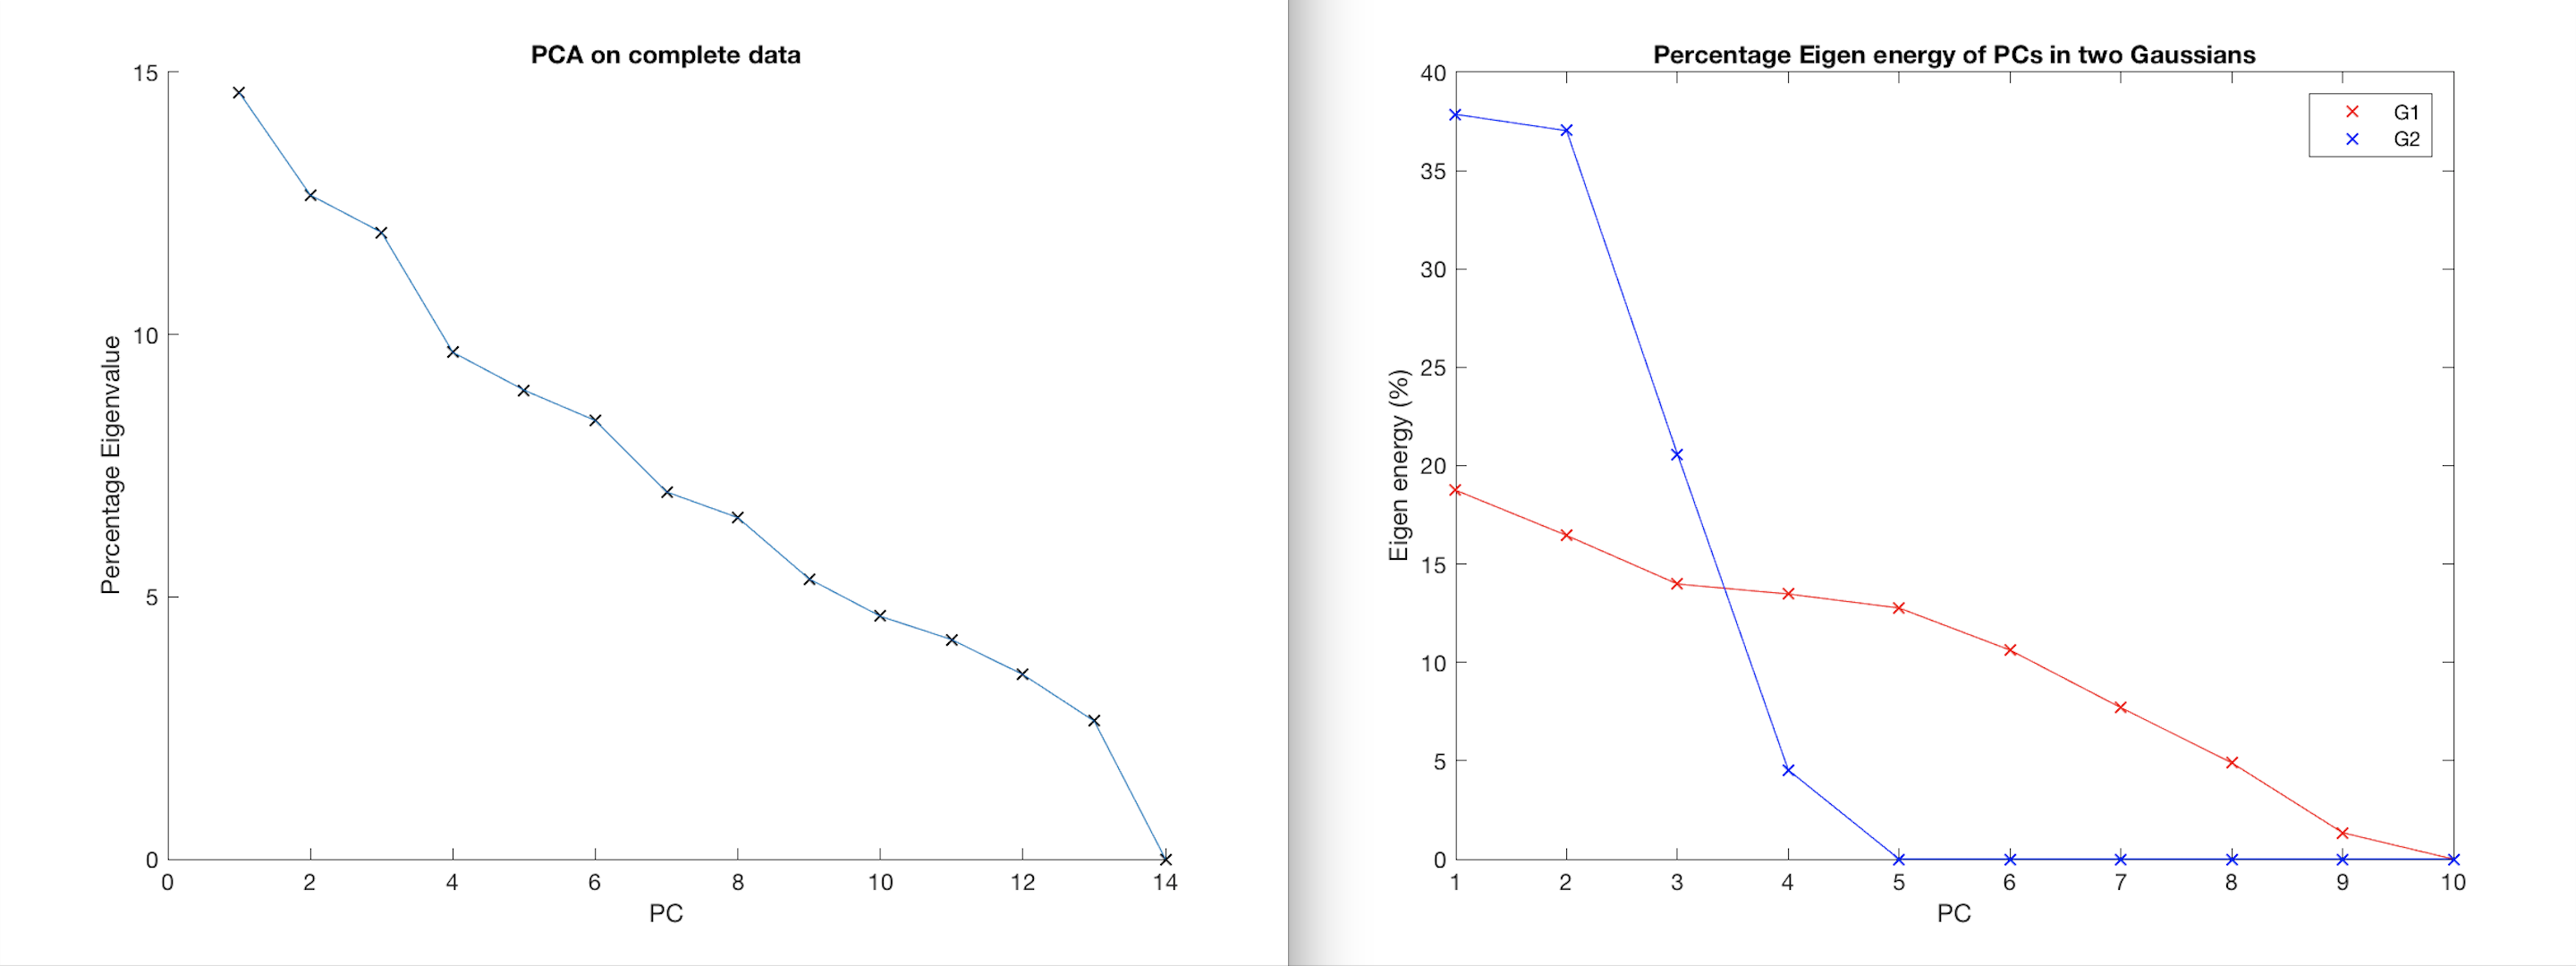
\includegraphics[width = 10cm]{splitpca}
				\centering
				\caption{For experts in clip 5, the explained variability of each principle component after PCA (left) vs. the explained variability of either of two Gaussians. The cut-off is generally set at 70\%, making PCA effective only after splitting the data.}
			\end{figure}
			On average, the first two Principal Components in at least one of two Gaussians for each clip, accounted for more than 70\% of the variability in that cluster \ref{fig:splitpca}, this being more than enough for ample dimensionality reduction at the cost of very little loss in information.
			\newpage
		\section{Classification}\label{results:class}
			The initial model used for classification in Single variable, Variable Pair and PCA space, before configuring hyperparameters, was built using a 3\textsuperscript{rd} order polynomial kernel function and a box constraint of 0.01. See \ref{approach:class:param}.
			\subsection{Single variable classification}\label{results:class:single}
				Out of 121 total variables for clips 1-6, 12 variables on average, or 10\%, produced models with less than 0.5 loss. With the mean validation loss being 0.8114. For a 2-class classification problem, random chance is 50\%. This can be considered quite a poor result, as it should be assumed that a classifier can do at least as good as random chance. Of the 12 variables that were better than random chance, 10 on average resulted in 70\% accuracy or better, a desirable accuracy for a classifier, 2 variables resulted in 100\% accuracy, or 0 loss. Given that each feature was measured 15 times over each clip, no feature was adequately classifiable throughout the clip. 
				
				For clips 7-14, there are 61 variables used for classification. Out of these 5 variables produced a model with accuracy better than random chance, with the mean loss being 0.8273. Only 3 variables succeeded at classifying better than 70\%, and most clips did not attain 100\% at all.	These are results very poor.
				
				As classifying on one variable is not sensible practically, and accounted for in this project given the large roster of features taken, the poor results of this test are not final, and an acceptable model was still attainable.

			\subsection{Pairwise classification}\label{results:class:pair}	
				\begin{figure}[h]\label{fig:pairwise}
					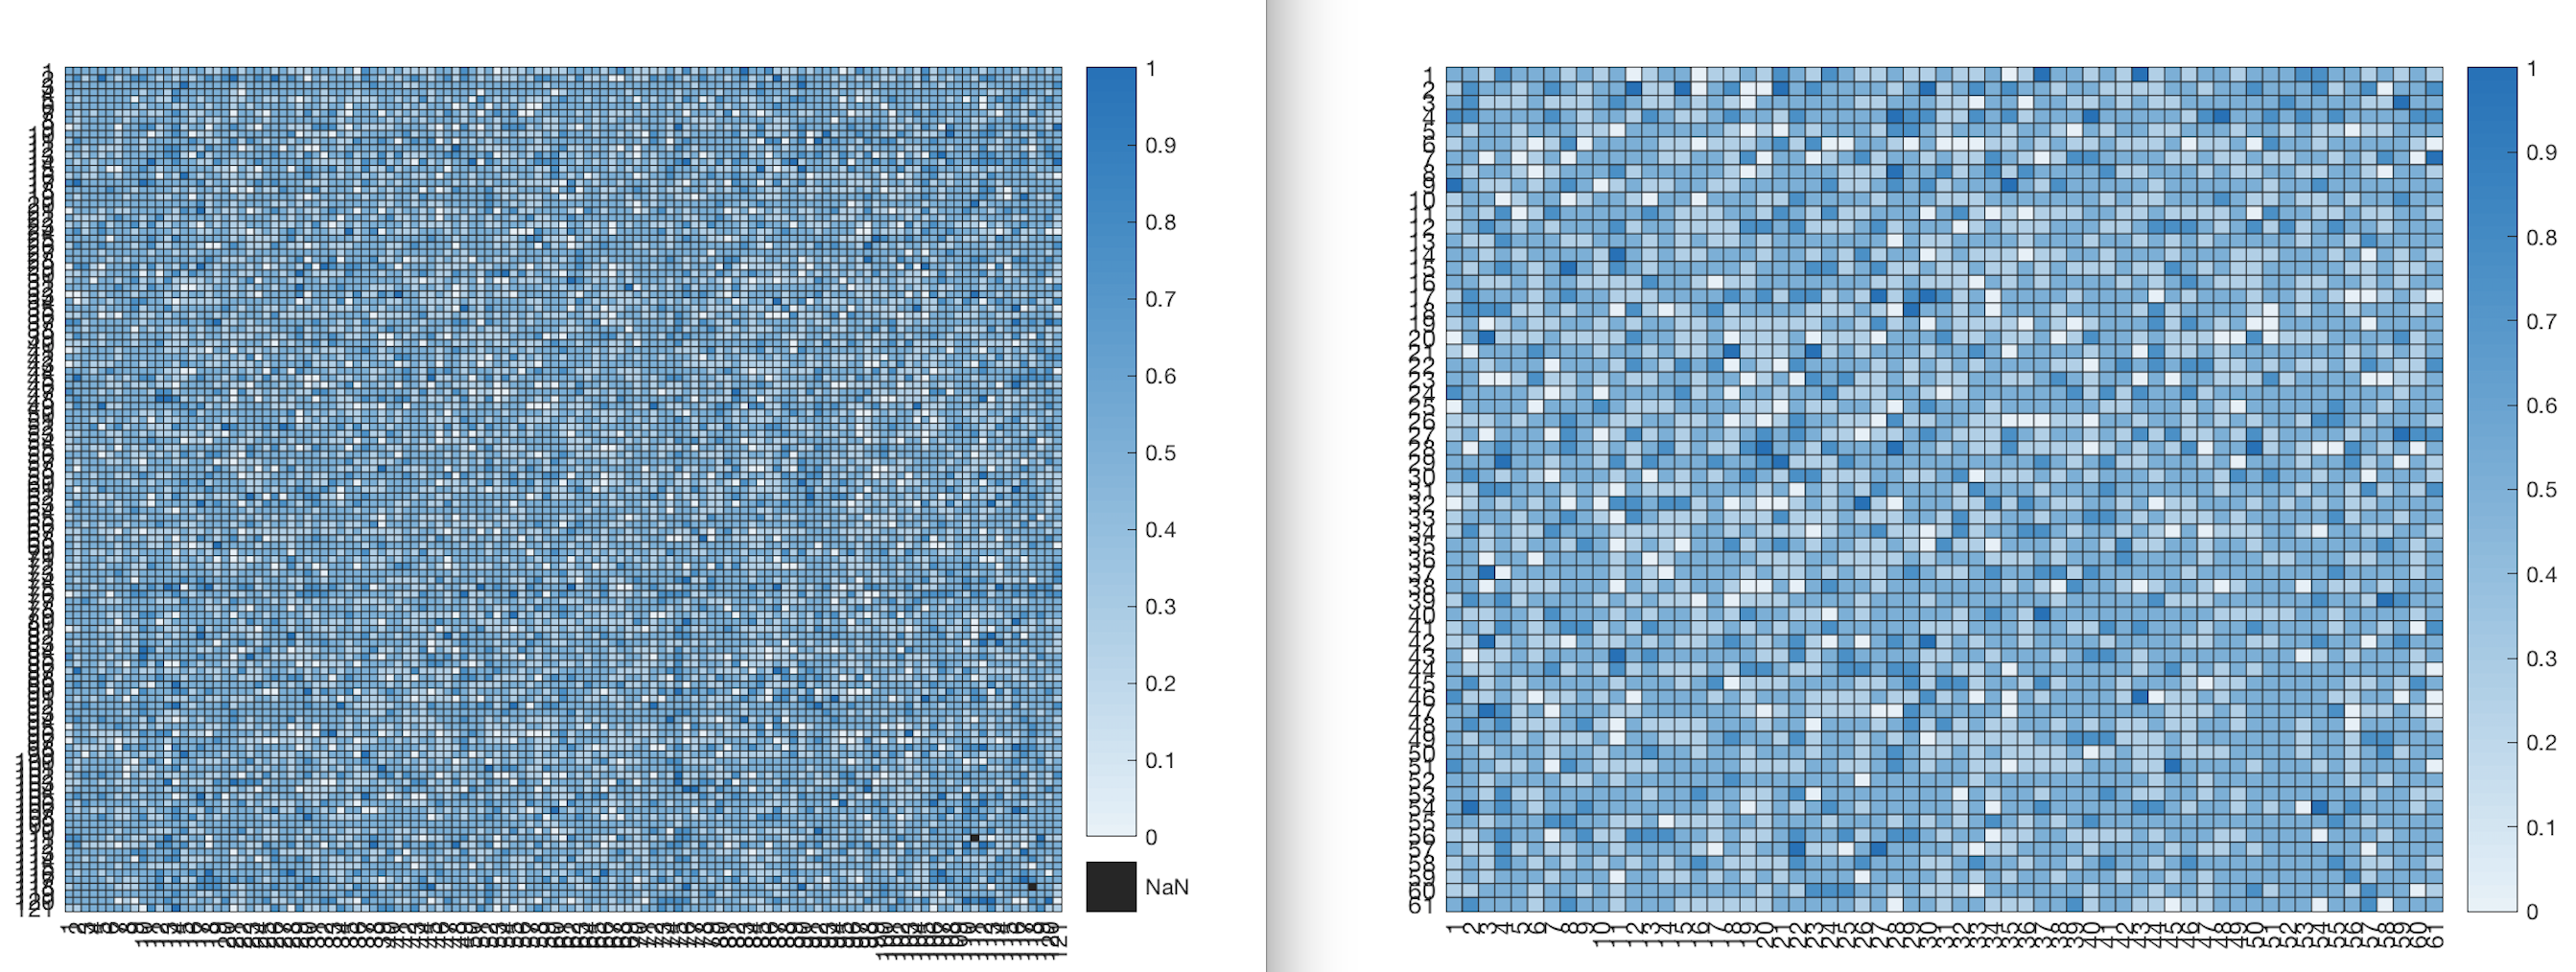
\includegraphics[width=12cm]{pairwise}
					\centering
					\caption{The results for 2-variable classification is overall positive for clip 5 (left), with a large population of medium-dark blue (60-100\% accuracy). Clip 10 (right) shows that many combinations result in approximately random chance, but some obtain a better more acceptable result.}
				\end{figure}			
				With 121 variables for image clip classification, and 61 for video clip classification, the first 6 clips were notably more computationally complex to generate heat maps for. As this test was mainly for visual evaluation of each clips potential for classification the resulting high resolution of the heatmaps made this slightly counterintuitive. However, from the figure it is clear that a conclusion can still be drawn for a clip\ref{fig:pairwise}.
				
				Results for all image clips were very similar to clip 5, and likewise for video clips to clip 10. The results of this test are slightly positive overall, considerably better than single variable classification. From these figures the feature space demonstrates the possibility for an effective model to be built, but it is also the case that no feature, represented by a contiguous set of 15 spaces, performs well over the whole clip, illustrating a necessity to include all features in order to avoid a reliance on any given segment of the clip for classification.
			\subsection{Sequential forward selection}\label{results:class:sfs}
			\begin{table}[h]
					\centering
					\caption{The results show a relatively low accuracy on average.\label{tab:sfs}}
					\begin{tabular}{|c|c|c|c|}
						\hline
						Clip & Sorted SFS & Un-sorted SFS & Sorted SBS\\
						\hline
						1 & 50.00\% & 50.00\% & 25\%\\
						\hline
						2 & 50.00\% & 50.00\% & 50.00\%\\
						\hline
						3 & 50.00\% & 50.00\% & 0.00\%\\
						\hline
						4 & 50.00\% & 50.00\% & 25.00\%\\
						\hline
						5 & 50.00\% &50.00\% & 0.00\%\\
						\hline
						6 & 50.00\% & 50.00\% & 50.00\%\\
						\hline
						7 & 75.00\% & 50.00\% & 25.00\%\\
						\hline
						8 & 50.00\% & 50.00\% & 25.00\%\\
						\hline
						9 & 50.00\% & 50.00\% & 50.00\%\\
						\hline
						10 & 50.00\% & 50.00\% & 50.00\%\\
						\hline
						11 & 50.00\% & 50.00\% & 50.00\%\\
						\hline
						12 & 50.00\% & 50.00\% & 50.00\%\\
						\hline
						13 & 50.00\% & 50.00\% & 25.00\%\\
						\hline
						14 & 50.00\% & 50.00\% & 50.00\%\\
						\hline
					\end{tabular}
				\end{table}
				Sequential forward selection aims to sequentially add features from a feature space until the accuracy of the resulting model decreases. Intuitively, this method cannot result in a lower accuracy than the lowest accuracy of the features selected, but instead by combining features the aim is to improve the accuracy of the model. It is unreasonable to expect a large improvement on the results of the single or pair classification results, that being said, an effective model is still possible from a combination of variables in some of the easier clips to classify. 
				
				As mentioned in \ref{approach:class:sfs}, in order to aid SFS, the features can be sorted in descending order of single classification accuracy so that the best feature for single classification is the first one evaluated by the algorithm and so on.
				The results are as expected not exceptionally better than any one of the variables for the clip. Surprisingly the results are for the vast majority 50\% accuracy \ref{tab:sfs}. This remains the same after being tested multiple times, which is even more unlikely given that \texttt{sequentialfs} has some aspect of randomness in the partition of data it chooses. It is also worth noting that SFS consistently only selected one variable before ceasing it's search, the same result was also true for Sequential Backward Search which did not remove any variables. This incredibly unexpected result calls into question the functionality of the \texttt{sequentialfs} function. Nonetheless the model still stands to be improved by PCA and tuning hyperparameters.
				
			\subsection{Classification in PCA space}\label{results:class:pca}
				\begin{table}[h] 
					\centering
					\caption{Classification before and after oversampling shows that the number of observations was in fact too small to build a successful model.\label{tab:pca}}
					\begin{tabular}{ |c|c|c| }
						\hline
						\textbf{Clip} & \textbf{Original Classification} & \textbf{Oversampled Classification}\\
						\hline
						  Clip 1 & 47.22\% & 87.00\%\\
						\hline
						Clip 2 & 47.32\% & 85.00\%\\
						\hline
						Clip 3 & 75.00\% & 78.50\%\\
						\hline
						Clip 4 & 60.00\% & 82.50\%\\
						\hline
						Clip 5 & 45.00\% & 89.50\%\\
						\hline
						Clip 6 & 60.00\% & 75.00\%\\
						\hline
						Clip 7 & 59.82\% & 88.00\%\\
						\hline
						Clip 8 & 55.00\% & 91.00\%\\
						\hline
						Clip 9 & 55.00\% & 85.50\%\\
						\hline
						Clip 10 & 44.44\% & 85.00\%\\
						\hline
						Clip 11 & 60.00\% & 91.00\%\\
						\hline
						Clip 12 & 53.57\% & 87.00\%\\
						\hline
						Clip 13 & 50.00\% & 86.50\%\\
						\hline
						Clip 14 & 60.00\% & 89.00\%\\
						\hline
						Avg. & 55.17\% & 85.75\%\\
						\hline
					\end{tabular}
				\end{table}

				PCA space will include all features transformed such that variance is maximised. Given for all clips each PCA was split into Gaussians, the result for each clip is the average loss over both models.

				The results \ref{tab:pca} were as expected given the poor performance in feature space. The PCA provided some improvement on the features by stretching out variability in them, but a massive improvement in results is not only unlikely, but also unexpected. With average accuracy being approximately 55\%, the demonstrated result is that the experts and non-experts recorded for this experiment are not different enough for accurate classification.
								
				However, as suggested in \ref{approach:dataquality}, this may be due to the lack of observations, as in \ref{approach:class} and later implemented in \ref{approach:class:pca}, oversampling the data results in much better classification accuracy. With 200 samples the penalty for missing 1 point from the original observations, which now falls at the centre of a cluster of points will be approximately 3.33\% rather than 6.67\%. A more acceptable sample space will also give the model a more defined region for both groups, even if those regions overlap. It can also be reasoned that as the points generated are very near to the original points, the model trained will still be trained on expert-like and non-expert-like observations. Effectively it is unlikely that oversampling the data will result in the model being considerably rewarded for classifying observations that are not realistic representations of either group. 
				
				\subsection{Configuring SVM hyperparameters}\label{results:class:param}
					The results collected after oversampling the data demonstrate an effective model for classification. The model still stands to be improved however. By changing the kernel function and box constraint as described in \ref{approach:class:param} the model can be significantly improved.
					\subsubsection{Kernel function}\label{results:class:param:kf}
						As stated in the documentation for fitcsvm \ref{impl:toolbox:statsandml:class}, the Gaussian kernel function is suited for one-class classification. In this scenario classification is between the class and an 'outlier' class. As in this problem we have two distinct classes, tests were only performed on Linear and Polynomial kernel functions. The polynomial kernel function requires that an order be specified. For this data, 3\textsuperscript{rd}, 4\textsuperscript{th} and 5\textsuperscript{th} order polynomials were evaluated.
						\begin{table}[h]
							\centering
							\caption{Accuracy is highest when using a 3\textsuperscript{rd} order polynomial kernel function \label{tab:kf}}
							\begin{tabular}{|c|c|c|c|c|}
								\hline
								\textbf{Clip} & \textbf{Linear} & \textbf{3\textsuperscript{rd} Order} & \textbf{4\textsuperscript{th} Order} & \textbf{5\textsuperscript{th} Order}\\
								\hline
								1 & 75.00\% & 91.50\% & 85.50\% & 65.00\%\\
								\hline
								2 & 87.00\% & 91.50\% & 92.50\% & 65.00\%\\
								\hline
								3 & 87.50\% & 90.50\% & 87.50\% & 53.50\%\\
								\hline
								4 & 81.00\% & 90.00\% & 73.00\% & 41.50\%\\
								\hline
								5 & 91.50\% & 98.00\% & 97.50\% & 64.00\%\\
								\hline
								6 & 78.00\% & 95.00\% & 77.00\% & 81.50\%\\
								\hline
								7 & 88.00\% & 91.50\% & 87.00\% & 62.00\%\\
								\hline
								8 & 69.00\% & 92.50\% & 94.50\% & 74.00\%\\
								\hline
								9 & 67.00\% & 88.50\% & 87.50\% & 60.50\%\\
								\hline
								10 & 73.00\% & 84.00\% & 79.50\% & 69.00\%\\
								\hline
								11 & 62.50\% & 93.00\% & 91.50\% & 84.50\%\\
								\hline
								12 & 67.50\% & 88.00\% & 86.50\% & 75.50\%\\
								\hline
								13 & 64.50\% & 75.00\% & 78.00\% & 74.50\%\\
								\hline
								14 & 63.50\% & 90.00\% & 88.00\% & 71.50\%\\
								\hline
								Avg. & 75.36\% & 89.93\% & 86.11\% & 67.29\%\\
								\hline
							\end{tabular}
						\end{table}
						All results are much better than the un-padded model, with the 3\textsuperscript{rd} polynomial kernel function having the best effect on the data by a small margin \ref{tab:kf}. Even the worst performing model, 5\textsuperscript{th} order polynomial, is more than acceptable for most clips, with the exception being Clip 3 and Clip 4 in which the model does very poorly.
		
					\subsubsection{Box Constraint}\label{results:class:param:bc}
						Given the exceedingly positive results from the 3\textsuperscript{rd} order polynomial kernel function, tests for different Box Constraints will all use this kernel function. Training a model with a higher box constraint will result in less misclassification in the training set. As a result, classification on average should be worse \ref{tab:bc}.
						\begin{table}[h]
							\caption{Tuning the box constraint gives a small increase in classification accuracy, with 0.001 averaging very slightly higher than 0.01 \label{tab:bc}}
							\begin{tabular}{|c|c|c|c|c|c|c|c|}
								\hline
								 Clip & \multicolumn{7}{c|}{Box Constraint}\\
								 \hline
								 & 10\textsuperscript{-4} & 10\textsuperscript{-3} & 10\textsuperscript{-2} & 10\textsuperscript{-1} & 10\textsuperscript{0} & 10\textsuperscript{1} & 10\textsuperscript{2}\\
								 \hline
								 1 & 94.00\% & 93.00\% & 91.50\% & 91.00\% & 90.50\% & 90.50\% & 90.50\%\\
								 \hline
								 2 & 94.00\% & 92.50\% & 91.50\% & 91.50\% & 91.50\% & 91.50\% & 91.50\%\\
								 \hline
								 3 & 91.00\% & 92.00\% & 90.50\% & 87.00\% & 88.00\% & 86.50\% & 86.00\%\\
								 \hline
								 4 & 89.50\% & 91.00\% & 90.00\% & 89.00\% & 88.50\% & 88.00\% & 88.50\%\\
								 \hline
								 5 & 98.50\% & 98.00\% & 98.00\% & 98.00\% & 98.00\% & 98.00\% & 98.00\%\\
								 \hline
								 6 & 92.00\% & 92.50\% & 95.00\% & 95.00\% & 95.00\% & 95.00\% & 95.00\%\\
								 \hline
								 7 & 94.00\% & 95.50\% & 91.50\% & 90.50\% & 90.50\% & 90.50\% & 90.50\%\\
								 \hline
								 8 & 93.50\% & 94.00\% & 92.50\% & 91.50\% & 91.50\% & 91.50\% & 91.50\%\\
								 \hline
								 9 & 82.50\% & 84.50\% & 88.50\% & 90.00\% & 87.00\% & 85.50\% & 84.50\%\\
								 \hline
								 10 & 76.00\% & 83.00\% & 84.00\% & 83.00\% & 81.50\% & 78.00\% & 73.50\%\\
								 \hline
								 11 & 93.50\% & 96.00\% & 93.00\% & 93.00\% & 90.50\% & 90.50\% & 90.50\%\\
								 \hline
								 12 & 84.00\% & 84.00\% & 88.00\% & 87.00\% & 85.50\% & 87.00\% & 86.00\%\\
								 \hline
								 13 & 76.00\% & 76.00\% & 75.00\% & 74.50\% & 77.00\% & 78.00\% & 79.00\%\\
								 \hline
								 14 & 85.50\% & 88.00\% & 90.00\% & 85.00\% & 85.50\% & 84.00\% & 84.00\%\\
								 \hline
								 Avg. & 88.86\% & 90.00\% & 89.93\% & 89.00\% & 88.61\% & 88.18\% & 87.79\%\\
								 \hline
							\end{tabular}
						\end{table}
		\section{Results evaluation}\label{results:eval}
			In general, the subjects' gaze clustered quite well into distinct areas within the scene. Each cluster in any image could be associated with a corresponding object or group of objects within the scene. Although clustering for the non-experts was less defined and more blurry, the overall results of clustering the data for image clips proved the method to be a reliable one for defining objects in the scene, and matching a subjects gaze with that object(s). Video clips did suffer considerably in this approach as a large portion of the screen featured moving objects, leading the subjects gaze along a large area, resulting in poor clustering without the temporal information.
			
			Feature extraction was also fruitful, with 10 identifiable features being measured from the data, 9 of which were used in the classification model for image clips. Increasing the dimensionality of the data initially, by measuring the features multiple times over the image, aided greatly in solving the later found problem of features being weak in certain sections of the clip. By separating each feature into a set of features, one for each section, weak areas could then be filtered without ruling out the feature wholly, which could still be useful towards, say, the beginning of the clip. As explained, the video clips did not provide defined cluster data, and as a result features with a focus on clustering were not used. This effectively ruled out 4 features for use with video clips.
			
			Dimensionality reduction is perhaps the least successful area of evaluation for this data set. When visualised by t-SNE using 3 popular distance measures, the data seemed inseparable in 2 of these different views, even in 3 dimensions. Where t-SNE, a non-linear, very powerful dimensionality reduction method which has been shown to be much more successful than other methods \cite{tsne}, fails, it is very unlikely that PCA, a less complex method might succeed. 
			
			The results of PCA show that dimensionality could not be effectively reduced back down without losing a significant portion of the data's variability. It was through testing the hypothesis that the data might be split into two clusters with variability in contrasting dimensions, that it was eventually proven that this was the case. Once the principle component data were split into Gaussians and measured, the following results were much more favourable. Variability in either cluster was shown to be heavily skewed to the first few principle components, allowing a lot of extra dimensionality to be discarded. This method is easily reproducible on new data, given the coefficients of the PCA, which would be used to transform the data from feature space, and the original mixture model, which can sort data into either of two clusters based on it's explained variability.
			
			Classification reflected the results of t-SNE, with the base model struggling to consistently classify better than random chance on the majority of variables. However, as explained in \ref{results:single}, this approach is not practical for a final model given each variable only accounts for 1 measure during 1 second  of a 15 second clip. So these results were not absolute. 
			
			Combining variables into pairs and classifying was again mainly an endeavour in visualising the classification space, and the possibility of an effective model built on a larger number of features. The use of colour to denote accuracy was very useful in defining regions of successful vs. unsuccessful feature pairs. While the majority of features in the earlier clips, 1-6, averaged at around 60\%, there was no region spanning 15 or more spaces, equal to a feature measured over the entirety of the clip, that kept above this boundary. This means that no feature could be relied on to be effective throughout the clip. Heat maps for video clips displayed a less successful overall classification using feature pairs. Each heat map was heavily dotted with light blue to white spaces, evidence of less than 50\% accuracy. 
			
			The results of single and pair classification were ambiguous in their prediction of the accuracy of a fuller model, built on a larger number of features. With the feature space translating relatively poorly into principle component space, and as a result the necessity to classify two subgroups of subjects formed from the clusters, expected success of the model was low. Classification on principle component scores was mixed, with some clips showing 60\%+ accuracy, but most being on par with random chance, or worse even. While splitting the scores into Gaussian clusters had allowed for a reasonable amount of dimensionality reduction, the classification in either subgroup was still quite poor.
			
			The poor results of SFS, assuming the Matlab implementation did work as intended, confirm that in feature space an effective model cannot be built given the features collected. Instead PCA would have to be used in order to maximise variability, in the hopes that this might give the model enough space to find an acceptable separation between the groups.
			
			In a final attempt to obtain an acceptable model, the principle component scores were oversampled. With approximately 180 extra observations to train on, all forming clusters around the original observations, the model fared much better. Accuracy was considerably improved after oversampling, such that all clips were at least 80\% in accuracy, with the exception of clip 6 which was still more than acceptable. 

			Following the vast improvement from oversampling the final step was to tweak hyperparameters in the hopes of slightly improving the accuracy for an optimal result. Concerning the kernel function, 3\textsuperscript{rd} order polynomial was by a small margin the best function to use. This follows a lucky estimation that lead to this kernel function being used prior to tuning, for the previous tests. Realistically, 3\textsuperscript{rd} order, 4\textsuperscript{th} order or even linear kernel functions all produced very high accuracies, with the only notably poor performance coming from 5\textsuperscript{th} order polynomial. In terms of value used for the box constraint, most values again produced similarly acceptable results. On average a value of 0.001 provided the best results at approximately 90\%, however, the highest record accuracy of any test was obtained using 0.0001, for clip 5 at 98.50\%.		
			
	\chapter{Conclusion}\label{concl}
		Overall, results for this project are very positive. The high classification accuracy for oversampled principle component data, as a feasible result for future use, is validated by previous tests. The reliability of the features used, at least for image clips, is validated by the clear clustering seen using GMMs \ref{approach:datavis:clustering}. The decision to reduce the dimensionality of the data via PCA is justified twofold: classification on any combination of original features was very poor, sometimes worse than random chance. For this reason, in tandem with the observation that no feature was consistently effective over the whole clip, meant that a model in original feature space would be high in dimensionality. Thus, the need for dimensionality reduction. Finally, given that the assertions that classification on oversampled data are sound, the model was vastly improved upon as a result of oversampling. This result aids concerns that the test scenario might not be an effective one.
		
		For reproducibility, a subject is recorded using any eye tracking camera, at the distance specified in \ref{approach:ftextrac:fixationdef}. The gaze data is then fitted to the clusters in the Gaussian Mixture Model fitted to the expert data. The features specified in \ref{approach:ftextrac:spatialft} and \ref{approach:ftextrac:temporalft} are then measured for this subject. Using the PCA coefficients for the clip, the measured data can be transformed into principle component scores. The PC scores are then fitted into one of two clusters, using the GMM trained on PC data for that clip. Finally, using either of the two models with the Statistics and Machine Learning Tooblox' matlab \texttt{predict} function will result in the models prediction for this subject.
		\section{Reflection on Learning}\label{concl:reflec}
			As a result of this project I have gained my first insight into Machine Learning. Machine learning has been an interest for me in some ways for longer than Computer Science. Through trial and error with one of the more powerful machine learning models, I have been able to learn the appropriate training, validation and evaluation methods for different scenarios. I have gained a comprehensive knowledge in Support Vector Machines, their inner workings and the hyper parameters tailored to each specific scenario. I have also become familiar with the field of eye tracking and the processing that converts this into model trainable data. Equally as important is the experience I have gained with professional research practice standards, on proper experiment techniques and report construction and writing. I finish this project feeling confident and informed for the research field, one that I am very hopeful to contribute more to.
		
	\chapter{Future Work}\label{future}
		While the project was an overall success, the results could be built upon in many different ways. For instance, the final results, while positive, relied heavily on oversampling of the data. The validity of these results has been proven to be very likely, but testing on a much larger data set of real observations is necessary to concretely confirm the theory. Given a larger data set, it would also be worthwhile evaluating the performance of other machine learning models on the data set. To name one such model, Recurrent Neural Networks using Long Short-Term Memory layers would make for an interesting approach to the problem. With a heavy focus on hidden temporal relations, LSTM RNNs could result in a generalised model for experts and non-experts, across all clips, rather than a GMM for clustering, and for PC data, and possibly two models for classification. This would be much more implementable at the cost of interpretability.
		
		The reproducibility of the models used in this project allow for implementation of software that uses such models for evaluation of medical personnel. Perhaps in a training environment, trainees could be asked to carry out the exercise, and their gaze data submitted to the model. If a trainee is following the correct procedure, or at least has had ample experience with the scenarios depicted in each clip, it follows that they should view the scene in a similar manner to the experts used in this project to train the resulting models. One such application of this, is in underdeveloped areas, where expensive medical training and equipment, as well employment costs for medical professionals to oversee training exercises, are not readily available. In the place of these resources, trainee medical staff could be evaluated by these models, and with some extension into explainability of these models, a membership function could produce as a result the degree to which that trainee fits the expert model.
		
		Possibly the most promising application of these results however, is the extensibility of the conclusion. The scenario described in this problem, of an expert analysing a scene, and the features taken, are not unique to anaesthetics. With some further testing in other non-medical fields, the same hypothesis could be proven for experts as a whole, providing valuable insight into the process by which someone gains expertise in a field, at least one in which this person is required to analyse a scene.
		
	\addcontentsline{toc}{chapter}{Bibliography}
	\begin{thebibliography}{11}
	\bibitem{gazecontrol}
	Henderson, J., (2003)
	\textit{Human gaze control during real-world
scene perception}
	TRENDS In Cognitive Sciences
	\bibitem{analyzingeye}
	Alam, S. and Jianu, R. (2017).
	\textit{Analyzing Eye-Tracking Information in Visualization and Data Space: From Where on the Screen to What on the Screen.}
	\bibitem{surgicaleye}
	Ahmidi, N., Hager, G., Ishii, L., Fichtinger, G., Gallia, G. and Ishii, M. (2010). 
	\textit{Surgical Task and Skill Classification from Eye Tracking and Tool Motion in Minimally Invasive Surgery.}
	Medical Image Computing and Computer-Assisted Intervention ? MICCAI 2010, pp.295-302.
	IEEE Transactions on Visualization and Computer Graphics, 23(5), pp.1492-1505.
	\bibitem{ecgeye}
	Davies, A., Brown, G., Vigo, M., Harper, S., Horseman, L., Splendiani, B., Hill, E. and Jay, C. (2016). 
	\textit{Exploring the Relationship Between Eye Movements and Electrocardiogram Interpretation Accuracy.}
	Scientific Reports, 6(1).
	\bibitem{expertpattern}
	Loveday, T., Wiggins, M., Festa, M., Schell, D. and Twigg, D. (2013).
	\textit{Pattern Recognition as an Indicator of Diagnostic Expertise.}
	Pattern Recognition - Applications and Methods, pp.1-11.
	\bibitem{eyemovements}
	Purves D, Augustine GJ, Fitzpatrick D, et al., (2001).
	\textit{Types of Eye Movements and Their Functions 2\textsuperscript{nd} edition}
	Sunderland (MA): Sinauer Associates.
	\texttt{https://www.ncbi.nlm.nih.gov/books/NBK10991/}
	\bibitem{tobii}
	\textit{How do Tobii Eye Trackers work?}
	\texttt{https://bit.ly/2I7puKR}
	\bibitem{curse}
	Keogh E., Mueen A. (2017).
	\textit{Curse of Dimensionality.}
	In: Sammut C., Webb G.I. (eds) Encyclopedia of Machine Learning and Data Mining. 
	Springer, Boston, MA
	\bibitem{eyeclustering}
	Blascheck, T., Kurzhals, K., Raschke, M., Burch, M., Weiskopf, D., Ertl, T. (2014).
	\textit{State-of-the-Art of Visualization for Eye Tracking Data}
	Eurographics Conference on Visualization (EuroVis)
	\bibitem{clustering}
	Jain, A.K. and Dubes, R.C., (1988).
	\textit{Algorithms for clustering data.}
	\bibitem{dimred}
	Van Der Maaten, L., Postma, E. and Van den Herik, J., (2009). 
	\textit{Dimensionality reduction: a comparative review.} 
	J Mach Learn Res, 10, pp.66-71.
	\bibitem{supervisedml}
	Kotsiantis, S.B., (2007).
	\textit{Supervised Machine Learning: A Review of Classification Techniques}
	Emerging Artificial Intelligence Applications in Computer Engineering, 3-15
	\bibitem{multilabel}
	Tsoumakas, G., Katakis, I., (2006)
	\textit{Multi-Label Classification: An Overview}
	Data Warehousing and Mining: Concepts, Methodologies, Tools, and Applications, ch 1.21
	\bibitem{svms}
	Hearst, M.A., Dumais, S.T., Osuna, E., Platt, J. and Scholkopf, B., (1998).
	\textit{Support vector machines.}
	IEEE Intelligent Systems and their applications, 13(4), pp.18-28.
	\bibitem{vapnik-svms}
	Cortes C., Vapnik V., (1995)
	\textit{Support-vector networks}
	Machine Learning 20(3),
	Springer
	\bibitem{ameen}
	Ul-Haq, A., (2015)
	\textit{Can we detect expert and novice anaesthetics by how they watch video?}
	Cardiff University
	\bibitem{effectofdataset}
	Brain D.,  Webb G., (2000)
	\textit{On the effect of data set size on bias and variance in classification learning}
	Proceedings of the Fourth Australian Knowledge Acquisition Workshop. 
	\bibitem{oversampling}
	Chawla, N.V., (2009).
	Data mining for imbalanced datasets: An overview. In Data mining and knowledge discovery handbook (pp. 875-886). Springer, Boston, MA.
	\bibitem{hmm}
	Schuster?B�ckler, B. and Bateman, A., (2007).
	\textit{An introduction to hidden Markov models.}
	Current protocols in bioinformatics, 18(1), pp.A-3A.
	\bibitem{kmeans}
	Lloyd, S. P. (1957)
	\textit{Least square quantization in PCM}
	Bell Telephone Laboratories Paper. 
	Published in journal much later: Lloyd., S. P. (1982).
	\bibitem{gmms}
	Nabney, I. T., (2004)
	\textit{NETLAB: Algorithms for Pattern Recognition}
	Springer, ch. 3
	\bibitem{elbow}
	Kodinariya, T.M. and Makwana, P.R., (2013).
	\textit{Review on determining number of Cluster in K-Means Clustering.}
	International Journal, 1(6), pp.90-95.
	\bibitem{overtva}
	O. Le Meur, et al., (2010)
	\textit{Overt visual attention for free-viewing and quality assessment tasks Impact of the regions of interest on a video quality metric}
	Elsevier
	\bibitem{tsne}
	van der Maaten L., Hinton G., (2008)
	\textit{Visualising Data using t-SNE}
	Journal of Machine Learning Research 9 2579-2605
	\bibitem{pca}
	Abdi H., Williams L. J., (2010)
	\textit{Principal Component Analysis}
	WIREs Comp Stat, 2: 433-459. 
	\bibitem{sfs}
	Marcano-Cede�o A., Quintanilla-Dom�nguez J., Cortina-Januchs M.G., Andina D., (2010)
	\textit{Feature selection using Sequential Forward Selection and classification applying Artificial Metaplasticity Neural Network}
	IEEE
	\bibitem{oneclasswGaussian}
	Chen Y. Q., Zhou X., Huang T. S., (2001)
	\textit{One-class SVM for learning in Image Retrieval}
	IEEE Conference on Image Processing
	\bibitem{matlab}
	MATLAB
	\texttt{https://uk.mathworks.com/products/matlab.html}
	\end{thebibliography}
\end{document}
